%!TEX outputDirectory = build
\documentclass[unicode, 12pt, a4paper, oneside, fleqn]{article}
\usepackage{styles/main}

\begin{document}
\tableofcontents 		% оглавление
\pagebreak
% Сюда инклюдить все небходимое!
% Матан
%!TEX root = ../report.tex"
\section{Вопрос 1: Непрерывность действительных функций одного и многих действительных переменных. Свойства непрерывных функций.}

\begin{defs}[Понятие функции]
Говорят, что на множестве $X$ имеется функция со значениями в $Y$, если в силу некторого $f$ каждому элементу $x \in X$ соответствует элемент $y \in Y$. Обозначается: $f: X \to Y$

$$f(x) := \{ y \in Y \ | \ \exists \ x ((x\in X) \wedge (y = f(x))) \} $$
\end{defs}


\begin{defs}[Предел по коши]
	Пусть $E \subset \Real$ и $f: E \to \Real$. Значение $A$ функции $f(x)$ в точке $x_0$ называется \underline{пределом}, если:
	$$\lim_{x\to x_0} f(x) = A \ \tittg \ \forall \varepsilon > 0 \ \exists \delta > 0: \forall x \ 0 < \Modul{x - x_0} < \delta \ \sledue \ \Modul{f(x) - a} < \delta$$
\end{defs}

\begin{defs}[Непрерывность в точке]
	Функция $f(x)$ называется непрерывной в точке $x_0$, если $\predel{x \to x_0}f(x) = f(x_0)$
\end{defs}

\begin{defs}[Определение непрерывности по Гейне]
	Говорят, что функция действительного переменного $f(x)$ является непрерывной в точке $a \in \Real$ если для любой последовательности $\{x_n\}$, такой что
	$$\lim_{n \to \infty}x_n = a, \text{выполняется соотношение} \lim_{n \to \infty}f(x_n) = f(a)$$
\end{defs}

\textbf{На практике удобно использовать следующие 3 условия} непрерывности функции $f(x)$ в точке $x = a$ (которые должны выполняться одновременно):
\begin{enumerate}
	\item Функция $f(x)$ определена в точке $a$
	\item Предел $\predel{x \to a}f(x)$ существует
	\item Выполняется равенство $\predel{x \to a}f(x)= f(a)$
\end{enumerate}

\begin{defs}
	Элементами пространства $\Rmern{n}$ являются упорядоченные наборы $\myvect{1}{n}$, где $x_i \in \Real$
\end{defs}

\begin{defs}
	$\Rmern{n}$ векторное пространство над $\Real$ $\sledue$ $x + y = (x_1+y_1, \ldots, x_{n}+y_{n})$, $\lambda \cdot x = (\lambda \cdot x_1, \ldots, \lambda \cdot x_n)$
\end{defs}

\begin{defs}
	$e_i = (\underbrace{0, \ldots, 1,\ldots,0}_n^i)$, где $i = \overline{1,n}$ стандартый базис $\Rmern{n}$
\end{defs}

\begin{defs}
	\textbf{Скалярным произведением} называется $x,y \in \Rmern{n}$, $\skobk{x,y} = \summa{i=1}{n}x_i \tochka y_i$, \textbf{Нормой вектора} $\DModul{x} = (x,x)^{\frac{1}{2}}$, \textbf{Расстояние между элементами $\Rmern{n}$} $\rho(x,y)= \DModul{x-y}$
\end{defs}

\begin{defs}[Открытый шар]
	Пусть $x \in \Rmern{n}$, $r > 0$.

	Обозначим $U(x,r)$ = $\fskobk{y \in \Rmern{n} \ : \ \DModul{x-y} < r}$ -- открытый шар радиуса $r$
\end{defs}

\begin{defs}
	Множество $U \in \Rmern{n}$ называется открытым, если $\forall x \in U \ \exists \ r > 0 \ : \  U(x,r) \subset U$
\end{defs}

\begin{defs}
	Окрестностью точки $x \in \Rmern{n}$ называется любое открытое подмножество, содержащее данную точку $:$ $U(x)$
\end{defs}

\begin{defs}
	Пусть $f: E \to \Rmern{m}$, $E \in \Rmern{n}$, $x_0 \in \prokol{E}$. Говорят, что $\exists$ предел $f(x)$ при $x\to x_0$ по мн-ву $E$, равный $a \in \Rmern{m}$, если $\forall \ U(a) \ \exists \ U(x_0) \ \forall x \in \prokol{U}_{E}(x_0) \sledue f(x) \in U(a)$
	и обозначается $\predel{x \to x_0}f(x)= a$
\end{defs}

\begin{claim}[]
	Если $\predel{x\to x_0}f(x)=(a_1,\ldots,a_m)=a$, то $\forall k \in \overline{1,m} $ $\exists \predel{x \to x_0}f_k(x)=a_k$

	Верно и обратное, Где $f(x)=(f_1(x),\ldots,f_m(x))$ -- координатное представление функции $f(x)$

\end{claim}

\begin{defs}
	Пусть $f: E \to \Rmern{m}$, $E \in \Rmern{n}$, $x_0 \in E$ Ф-я $f(x)$ называется непрерывной в точке $x_0$, если $\forall U(f(x_0)) \ \exists U(x_0): \ \forall x\in U_E(x_0) \sledue f(x) \in U(f(x_0))$
	\begin{itemize}
		\item $x_0$ изолированная $\sledue$ $f(x)$ всегда непрерывна в точке $x_0$
		\item $x_0$ предельная точка $E$ $\sledue$ $\skobk{f(x) \text{ непрерывна в точке } x_0} \tittg \exists \predel{x \to x_0}f(x)=f(x_0)$
	\end{itemize}
\end{defs}

\begin{claim}
	Пусть $f: E \to \Rmern{m}$, $E \in \Rmern{n}$, $x_0 \in E$, $f(x)=(f_1(x),\ldots,f_m(x))$
	Тогда \fx непрерывна в точке $x_0$ $\tittg$ $\forall \ i = \overline{1,m}$ $f_i(x) \text{ непрерывна } в x_0$
	\begin{dokvo}
	Если $x_0$ - изолированная, то все доказано. Пусть $x_0 \in E$, тогда \fx непрерывна в точке $x_0 \ \tittg \ \exists \predel{x \to x_0}f(x)=f(x_0) \ \naverh{по утв}\tittg \ \exists \predel{x \to x_0}f_i(x) = f_i(x_0) \forall i = \overline{1,m}$
	\end{dokvo}
\end{claim}

\begin{claim}
	\begin{enumerate}
		\item $f_1,f_2: E \to \Rmern{m}$, $E \in \Rmern{n}$, $f_i$ непрерывна в точке $x_0 \in E$ $\sledue$ $f_1 + f_2, \lambda\cdot f_1$ непрерывны в точке $x_0$
		\item $f_1,f_2: E \to \Rmern{m}$, $E \in \Rmern{n}$, $f_i$ непрерывна в точке $x_0 \in E$ $\sledue$ $f_1 \cdot f_2, \frac{f_1}{f_2}$, если $f_2 \neq 0$
	\end{enumerate}

	\begin{dokvo}
		Следует из свойств предела функции
	\end{dokvo}
\end{claim}

\begin{defs}
	$f: E \to \Rmern{m}, \ E \subseteq \Rmern{n}$. Ф-я \fx \ называется непрерывной на $E$, если она непрерывна в любой точке множества $E$
\end{defs}

\begin{claim}
	Пусть $f(x):E \to J, E \subseteq \Rmern{n}, J \subseteq \Rmern{m}, \ g(y):J\to \Rmern{k}$

	$\left.\begin{array}{l}
		f(x) \text{ непрерывна в точке } x_0 \in E \\
		g(y) \text{ непрерывна в точке } y_0 \in f(x_0)
	\end{array}\right\} \sledue$ $g \circ f$ непрерывна в т. $x_0$

	\begin{dokvo}
		Зафиксируем любую $U(g(y_0))$ т.к $g(y)$ непрерывна в т. $y_0$, то $\exists U(y_0)=U(f(x_0)):\forall y \in U_y(y_0) \sledue g(y) \in U(g(y_0))$

		С другой стороны \fx непрерывна в точке $x_0\in E \sledue \exists U(x_0): \forall x\in U_E(x_0) \sledue g(x)\in U(f(x_0)) \sledue g(f(x))\in U(g(y_0))$

		То есть имеем: $\forall \ U(g(f(x_0))) \ \exists  \ U(x_0):\forall x\in U_E(x_0)\sledue g(f(x))\in U(g(f(x_0)))$
	\end{dokvo}
\end{claim}

\begin{defs}
	Множество $M \in \Rmern{n}$ называется компактным $\naverh{опр}\tittg$ из любого покрытия $M$ открытыми подмножествами можно выделить конечное подпокрытие.
\end{defs}

\begin{proofs}[1-я теорема Вейерштрасса про ограниченность непрерывной функции]
	Если ф-я $f: E \to \Rmern{m}$ непрерывна на $E$, $E$ - компактное подмножество $\Rmern{n}$, то $f$ -- ограничена. $f(E)$ ограниченное подмножество $\Rmern{n}$
	\begin{dokvo}
		$\forall x \in E$ $f$-непрерывна в точке $x$ $\sledue$ $\exists \ U(x,r_x) \ r_x > 0:\forall z \in E \peres U(x,r_k)$

		$\DModul{f(z)} \subseteq M_x$, $E \subset \bigcup\limits_{x \in E}U(x,r_x)$ $E$-компактно $\sledue$ можно выбрать конечное подпокрытие, т.е разбить $E \subset \bigcup\limits_{i = 1}^{k} U(x_i,r_{x_i})$, $M = \max\limits_{1 \leq i \leq k} M_{x_i}$ $\sledue \ \forall x \in E$ $\exists \ U(x_j, r_{x_j}): x \in U(x_j,r_{x_j}) \sledue \DModul{f(x)} \subseteq M_{x_{j}} \subseteq M$
	\end{dokvo}
\end{proofs}

\begin{proofs}[2-я теорема Вейерштрасса о достижении верхней и нижней границ]
	Пусть $f:E \to \Real$, $f$-непрерывна на $E$, $E$-компактное подмножество $\Rmern{n}$ Тогда $\exists \ x_1,x_2 : f(x_1)=\max\limits_{x \in E}f(x), \ f(x_2)=\min\limits_{x \in E}f(x)$
	\begin{dokvo}
		$f$-непрерывна на $E$ $\sledue$ по 1 теореме Вейерштрасса $f$ ограничена на $E$ $\sledue$ $\exists \sup\limits_{x\in E}f(x)=M\in \Real$

		Покажем, что $\exists x_1 \in E : f(x_1)=M$ Предположим противное и рассмотрим ф-ю $g(x) = \frac{1}{M-f(x)}$, $M-f(x)$ непрерывна и не $\neq 0 \ \sledue$ $g(x)$ непрерывна на $E$ и по 1-й теореме Вейерштрасса ограничена на $E$

		С другой стороны т.к. $M=\sup\limits_{x\in E}f(x)$, то $\exists \ \fskobk{x_k}: \predel{k\to \infty}f(x_k)=M \ \sledue \predel{k\to \infty}(M-f(x))=0 \ \sledue \predel{k\to \infty}\frac{1}{M-f(x)}=\infty$, \underline{противоречие} с тем что $g(x)$ ограничена

		\textbf{Для минимума также}
	\end{dokvo}
\end{proofs}

\begin{proofs}[Кантора о равномерной непрерывности]
	Пусть $f:E\to \Rmern{m}$, $f$ - непрерывна на $E$, $E$-компактое подмножество в $\Rmern{n}$. Тогда $f$ - равномерно непрерывна на $E$
	\begin{dokvo}
		$x \in E, \ \forall \epsilon > 0, \exists \delta_x > 0: \forall \ z\in U(x, \delta_x)\peres E: \DModul{f(x)-f(z)}< \frac{\epsilon}{2}$
		$E \subset \bigcup\limits_{x\in E}U\skobk{x_i,\frac{\delta_x}{2}}$ -- покрытие открытыми подмножествами $\sledue$ можно выбрать конечное подпокрытие $E \subset \bigcup\limits_{i=1}^{k}U\skobk{x_i,\frac{\delta_{x_{i}}}{2}}$

		Пусть $\delta = \min\limits_{1 \leq i \leq k}\frac{\delta_{x_{i}}}{2}$ и рассмотрим произвольные $x^{\shtrih},x^{\shtrih\shtrih} \in E: \DModul{x^{\shtrih} - x^{\shtrih\shtrih}} < \delta$ $\exists i_0: 1 \leq i_0 \leq k \ : x^{\shtrih} \in U\skobk{x_{i_0},\frac{\delta_{x_{i_0}}}{2}} \sledue$ $\DModul{x^{\shtrih} - x_{i_0}} < \delta_{x_{i_0}}$ $\sledue$ $\DModul{f(x^{\shtrih}) - f(x_{i_0})} < \frac{\epsilon}{2}$

		C другой стороны рассмотрим $x^{\shtrih\shtrih}:\DModul{x^{\shtrih\shtrih} - x_{i_0} }$
		$\leq$ $\DModul{x^{\shtrih\shtrih} - x^{\shtrih}} + \DModul{x^{\shtrih} - x^{i_0}} < \skobk{\delta + \frac{\delta_{x_{i_0}}}{2}} \leq \delta_{x_{i_0}}$ $\sledue$ $\DModul{f(x_{i_0}) - f(x^{\shtrih\shtrih})} < \frac{\epsilon}{2}$
	\end{dokvo}

\end{proofs}

\begin{defs}[равномерно непрерывная]
	Пусть $f: E \to \Rmern{m}, \ E \subset \Rmern{n}$, тогда $f$ называется равномерно непрерывной на $E \ \tittg \ \forall \epsilon > 0 \exists \ \delta > 0 : \forall x_1,x_2 \in E \ \DModul{f(x_1)-f(x_2)} < \frac{\epsilon}{2}$
\end{defs}

\begin{defs}[связное подмножество]
	Подмножество $E \in \Rmern{n}$ называется связным, если $\forall x_1, x_2 \in E \ \exists$ непрерывное отображение $\phi: \kskobk{0,1}\to E:$ $\phi(0)=x_1,\phi(1)=x_2$
\end{defs}

\begin{proofs}[Теорема Больцано-Коши]
	Пусть $f: E \to \Real$, $f$ непрерывна на $E$, $E$ -- связное подмножество в $\Rmern{n}$, $x,y \in E : f(x) < 0 < f(y)$. Тогда $\exists c \in E : f(c) = 0$
	\begin{dokvo}
		без доказательства
	\end{dokvo}
\end{proofs}

\begin{defs}[точки разрыва]
	$f: E \to \Real, E \subseteq \Real$, точка $x_0 \in \Real$ является точкой разрыва \fx, если
	\begin{enumerate}
		\item либо $\skobk{x_0 \in E} \I $ $\skobk{f - \text{не является непрерывной в точке} \ x_0}$
		\item либо $\skobk{x \notin E} \I \skobk{x \in \prokol{E}}$

	\end{enumerate}
\end{defs}

\begin{defs}[устранимая]
	$x_0 \in E$ называется устранимой точкой разрыва если:
	$$\skobk{x_0 \ \text{точка разрыва}} \I \skobk{\exists \predel{x\to x_0 \in E}f(x) = A \in \prokol{R}}$$
\end{defs}

\begin{defs}[I рода]
	Точка разрыва $x_0$ называется точкой разрыва \textbf{I рода} если:
	\begin{enumerate}
		\item $x_0 \in \prokol{E}^{+} \sledue \exists f(x_0 + 0) \naverh{обозн}\tittg \predel{x\to x_0 + 0 \ \in E}f(x) \ \in \Real$
		 \item $x_0 \in \prokol{E}^{-} \sledue \exists f(x_0 - 0) \naverh{обозн}\tittg \predel{x\to x_0 - 0 \ \in E}f(x) \ \in \Real$
	\end{enumerate}
\end{defs}

\begin{claim}
	Всякая устранимая точка разрыва является точкой разрыва \textbf{I рода}
\end{claim}

\begin{defs}
	Точка $x_0$ разрыва \fx называется точкой разрыва \textbf{II рода} если она не является точкой разрыва \textbf{I рода}\footnote{джиниусы блин}
\end{defs}

\begin{claim}[Свойства точки разрыва]
	$f(x): E \to \Real, E \subseteq \Real$

	$\left.\begin{array}{l}
		1) f(x) \text{ монотонна на E } x_0 \in E \\
		2) \skobk{a \in E} \I \skobk{\text{а точка разрыва}}
	\end{array}\right\} \sledue$ $а$ является точкой разрыва \textbf{I рода}
\end{claim}

\begin{defs}[Еще раз по Гейне, но только в терминах]
	$x_0 \in \prokol{E}$, говорят что $\predel{k\to\infty}f(x) = A$, если для $\forall \ \fskobk{x_k}: \predel{k\to \infty}x_k = x_0, \ x_k \in E, x_k \neq x_0, \forall k \in \Natural, \ \predel{k\to\infty}f(x_k) = A$
\end{defs}

\begin{example}[Пример на точку разрыва]

\end{example}
\newpage
 %Ванек
%!TEX root = ../report.tex"
\section{Вопрос 2: Дифференцируемость функций одного и многих действительных переменных
в точке и на множестве. Достаточное условие дифференцируемости.
Производные и дифференциалы высших порядков.}



\begin{defs}
	Отображение $L: \Rmern{n}\to\Rmern{m}$ называется линейным если:
	\begin{enumerate}
		\item $L(x+y)= L(x) + L(y), \ \forall x,y \in \Rmern{n}$
		\item $L(\lambda \cdot x) = \lambda \cdot L(x), \forall
		\lambda \in \Real,  x\in \Rmern{n}$
	\end{enumerate}

	\zagolovok{Свойства}
	\begin{enumerate}
		\item $x = (x_1, \ldots, x_n) \in \Rmern{n}$, $\overline{l} = (l_1,\ldots,l_n)$ -- стандартный базис $\Rmern{n}$ $x = \summa{i=1}{n}x_i \cdot l_i$ $\sledue$ $L(x) = \summa{i=1}{n}L(l_i)\cdot x_i$

		\item $\overline{f}= (f_1,\ldots,f_m)$ -- стандартный базис $\Rmern{m}$ $A_l = \skobk{L(l_1)^{\downarrow}_{\overline{f}},\ldots,L(l_m)^{\downarrow}_{\overline{f}}} \in \Real_{m \times n}$ -- матрица линейного отображения $\sledue$ $L(x) = \overline{f} \cdot A_l \cdot x_{\overline{l}}^{\downarrow}$
	\end{enumerate}
\end{defs}

\begin{defs}
	$f: U \to \Rmern{m}$, $U$ -- открытое подмножество в $\Rmern{n}, x_0 \in U$\footnote{Лучше про многомерные случаи не говорить, сложно не успеем}

	Будем говорить, что $f$ - дифференцируема в точке $x_0$, если $\exists$ линейное отображение $A: \Rmern{n} \to \Rmern{m}: \ f(x_o + h) - f(x_0)= A(h) + o(\DModul{h}), \ h \to 0$ тоесть обозначается $f(x_0 + h)-f(x_0)=Ah+o(h), h\to 0$ при этом $A$ называется производной отображения $f$ в точке $x_0$ и обозначается $f^{\shtrih}(x)$
\end{defs}

\begin{claim}[Свойства диференцируемых отображений и производной]
	\begin{enumerate}
		\item Если $f: U \to \Rmern{m}, U \subset \Rmern{n}$ -- открытое, дифференцируема в точке $x_0 \in U$, то $f$ - непрерывна в точке $x_0$
		\begin{dokvo}
			$\dprirash f = f(x_0 + h) - f(x_0)$, $\predel{h \to 0} \dprirash f = \predel{h \to 0}\skobk{f^{\shtrih}(x_0)h + o(h)}$ $\sledue$ $f$ непрерывна в точке $x_0$
		\end{dokvo}
	\end{enumerate}
\end{claim}

\begin{defs}
	$\pust f:E\to \Real, x \ $ - предельная точка множества $E$, тогда функция $f$ называется дифференцируемой в точке $x$, если $\exists \predel{\dprirash x \to 0}\frac{f(x+\Delta x)-f(x)}{\dprirash x}$, сам предел называется производной функции $f$ в точке $x$ и обозначается $f\shtrih(x)$

	Если $M \subset E$ и $f$ диф-ма в $\forall$ точке $x \in M$, то $f$ - дифференцируема на $M$

	Если $x$ предельная точка множества $E_{x-0} \ILI E_{x+0}$ и $\exists \predel{\Delta x \to -0 \ (+0)}frac{f(x+\Delta x)-f(x)}{\dprirash x}$, то этот предел - левая $\ILI$ правая производная $f^{\shtrih}_{\text{Л}} \ILI f^{\shtrih}_{\text{ПР}}$ в точке x
\end{defs}

\begin{proofs}[Переформулировка определения критерия дифференцируемости]
	$\pust f: E \to \Real$, т.$x$ предельная точка множества $E$, тогда $f$ - дифференцируема в \vtochke{x} $\tittg \ \exists A \in \Real$ и $f(x + \Delta x) - f(x)$ представимо в виде $A \tochka \Delta x + \overline{o}(\Delta x), \Delta x \to 0$, и в этом случае $A = f^{\shtrih}(x)$

	\begin{dokvo}
		Будем говорить, что ф-я \fx является $\overline{o}$ - функции $g(x)$, если $\exists$ такая бесконечно малая величина $\alpha(x): \ f(x) = \alpha(x) \cdot g(x)$, при $x \to x_0$ - предельная точка множества $E$
		\begin{itemize}
			\item[$\Rightarrow$] $\pust \ f$ -дифференцируема, тогда верно: $f^{\shtrih}(x) = \predel{\Delta x \to 0}\frac{f(x + \Delta x) - f(x)}{\Delta x} \ \sledue$ на языке $\mathsf{o}$--символики $= f^{\shtrih}(x) + \frac{f(x + \Delta x) - f(x)}{\Delta x} =\omaloe{1}$, $\dprirash x \to 0 | \cdot \Delta x \ \sledue$ $f(x + \dprirash x) - f(x) = \underbrace{f^{\shtrih}(x)}_{A} \cdot \Delta x + \underbrace{\omaloe{1} \cdot \Delta x}_{\omaloe{\Delta x}}$ $\sledue$ в одну сторону доказано.

			\item[$\Leftarrow$] $f(x + \Delta x) - f(x) = A \cdot \Delta x + \omaloe{\Delta x}$ делим на $\Delta x$ $\frac{f(x + \Delta x) - f(x)}{\Delta x} = A + \frac{\omaloe{\Delta x}}{\Delta x}$, $\omaloe{\Delta x} = 0$ по определению, $\Delta x \to 0 \ \sledue \predel{\Delta x \to 0}\frac{f(x + \Delta x) - f(x)}{\Delta x} = A + 0 \sledue \ A = f^{\shtrih}(x)$
		\end{itemize}
	\end{dokvo}
\end{proofs}

\begin{proofs}
	$\pust f \I g $ - дифференцируемы в \vtochke{x} $\sledue$
	\begin{itemize}
		\item $\skobk{f+g}$ - диф-ма в \vtochke{x} и $\skobk{f+g}^{\shtrih}(x) = f^{\shtrih}(x) + g^{\shtrih}(x)$
		\item $\skobk{f \cdot g}$ - диф-ма в \vtochke{x} и $\skobk{f \cdot g}^{\shtrih}(x) = f^{\shtrih}(x) \cdot g(x) + f(x) \cdot g^{\shtrih}(x)$
		\item Если $g(x) \neq 0$, то $\skobk{\frac{f}{g}}$ диф-ма \vtochke{x} и $\skobk{\frac{f}{g}}^{\shtrih}(x) = \skobk{\frac{f^{\shtrih}(x) \cdot g(x) - f(x) \cdot g^{\shtrih}(x)}{g^{2}(x)}}$
		\end{itemize}
	\begin{dokvo}
		Все три случая доказывать не нужно, лучше сразу доказать самый третий!\footnote{$\Delta f = f(x+\Delta x) - f(x)$}

		\begin{gather*}
			\skobk{\frac{f(x)}{g(x)}}^{\shtrih} \naverh{опр}= \predel{\Delta x \to 0}\frac{\Delta \skobk{\frac{f(x)}{g(x)}}}{\Delta x} = \predel{\Delta x \to 0}\frac{\frac{f(x + \Delta x)}{g(x+ \Delta x)} - \frac{f(x)}{g(x)}}{\Delta x} \ \naverh{предел суммы равен}\sledue \\
			\predel{\Delta x \to 0}\frac{f(x + \Delta x) \cdot g(x) - f(x) \cdot g(x + \Delta x)}{\Delta x \cdot g(x + \Delta x) \cdot g(x)} = \\ \frac{1}{g^{2}(x)} \cdot \predel{\Delta x \to 0} \frac{(f(x) + \Delta f(x)) \cdot g(x) - f(x) \cdot (g(x) + \Delta g(x))}{\Delta x} =\\
			\frac{1}{g^{2}(x)} \cdot \predel{\Delta x \to 0}\frac{f(x)\cdot g(x) + \Delta f(x)\cdot g(x) - f(x)\cdot g(x) - f(x)\cdot \Delta g(x)}{\Delta x} = \\
  	\end{gather*}

		\begin{gather*}
			\frac{1}{g^{2}(x)} \cdot \frac{g(x)\cdot \Delta f(x) - f(x) \cdot \Delta g(x)}{\Delta x} = \frac{1}{g^{2}(x)} \cdot \skobk{g(x) \cdot \predel{\Delta x \to 0}\frac{\Delta f(x)}{\Delta x} - f(x) \cdot \predel{\Delta x \to 0}\frac{\Delta g(x)}{\Delta x}} =\\
		= \skobk{\frac{f^{\shtrih}(x) \cdot g(x) - f(x) \cdot g^{\shtrih}(x)}{g^{2}(x)}}
		\end{gather*}
	\end{dokvo}
\end{proofs}

\begin{defs}
	Если $f$ - дифференцируема в \vtochke{x} $\sledue$ дифференциалом функции $f$ в \vtochke{x} с соответствующим приращением $\delt x$ называется линейная ф-я от приращения
	$$\delt f = f^{\shtrih}(x) \cdot \delt x = f^{\shtrih}(x)\pode{x}$$
\end{defs}

\begin{proofs}[Производная сложной функции]
	$f: E \to \Real, \ g:f(E) \to \Real$, $f$-дифференцируема в \vtochke{x} и $g$ - дифференцируема в \vtochke{y} $=$ \fx $\sledue$ композиция функций $(g \circ f)(x)$ дифференцируема в \vtochke{x} и $(g \circ f)(x) = g^{\shtrih}(y) \cdot f^{\shtrih}(x)$
	\begin{dokvo}
		Рассмотрим $(g \circ f)(x + \delt x)- (g \circ f)(x) = g(f(x + \delt x)) - g(f(x)) \oeq$

		$\pust \ \delt y=f(x + \delt x) - \underbrace{f(x)}_{=y}$, $\delt y \to 0$ при $\delt x \to$, т.к. $f$ -непрерывна в \vtochke{x}

		Так как если $f$ - дифференцируема в \vtochke{x} и $f(x+ \delt x)-f(x) = f^{\shtrih}(x)\delt x + \omaloe{\delt x}$

		$\oeq$ $g(y+ \delt y) - g(y) \naverh{из диф-ти g}= g^{\shtrih}(y)\cdot \delt y + \omaloe{\delt y} = g^{\shtrih}(f^{\shtrih}(x)\cdot \delt x + \omaloe{\delt x}) + \omaloe{\delt y}$ $= g^{\shtrih}(y)\cdot f^{\shtrih}(x)\delt x + \omaloe{\delt x} + \omaloe{\delt y}$

		Покажем что $\omaloe{\delt x} = \omaloe{\delt y}:$ по определению, $\omaloe{\delt y} = \alpha(\delt y) \cdot \delt y, \ \alpha(\delta y) \to 0$ при $\delt y \to 0$, можно считать, что $\alpha(\delt y) = 0$ при $\delt y = 0 \ \sledue$ при $\delt x \to 0 \ \alpha(\delt y) \to 0 \sledue \ \alpha(\delt y) = \omaloe{1}$ при $\delt x \to 0$ $\sledue$ $\omaloe{\delt y} = \omaloe{1}\cdot \delt y = \underbrace{\omaloe{1} \cdot (f^{\shtrih}(x)\delt x + \omaloe{\delt x})}_{\omaloe{\delt x}}$, $\delt x \to 0$
		$\sledue \ (g \circ f)^{\shtrih}(x)=g^{\shtrih}(y)\cdot f^{\shtrih}(x)\cdot \delt x + \omaloe{\delt x} \sledue$ $g \circ f$ - диффернцируема в \vtochke{x} и $(g \circ f)^{\shtrih}(x) = g^{\shtrih}(x) \cdot f^{\shtrih}(x)$
	\end{dokvo}
\end{proofs}

\begin{defs}[Высшие и производные и дифференциалы]
	Если функция \fx \ дифференцируема на $E$, а $f^{\shtrih}(x)$ имеет производную в \vtochke{x_0} $\in E$, то функция $f^{\shtrih}(x_0)$ называется второй производной функции $f$ в \vtochke{x_0} и обозначается $f^{\dshtrih}$

	Если $\exists$ $n$-я производная $f^{(n)}$ - функции $f$ на $E$ и $\exists$ $(f^{(n)})^{\shtrih}(x)$ \vtochke{x_0}, то она называется $(n+1)$ производной в \vtochke{x_0} и обозначается $f^{(n+1)}(x_0)$\footnote{Полагаем что -- $f^{(0)}=f(x)$}

	\zagolovok{Функция $n$-раз дифференцируема} означает, что $\exists \ n$ производных на множестве $E$ у этой функции и все они являются непрерывными.

	\zagolovok{Функция $\infty$-раз дифференцируема}  означает, что $\exists$ производная $\forall$ порядка для \vtochke{x_0} или $\forall$ точки из $E$
\end{defs}

\begin{proofs}[Теорема формула Ньютона-Лейбница]
	$\pust$ функции $u$ и $v$ - $n$-раз диффер-мы в \vtochke{x} $\sledue$\footnote{С помощью формулы Лейбница можно вычислить производную $n$-го порядка от произведения двух функций.}
	$$(u \cdot v)^{(n)}(x) = \summa{m=0}{n}\comb{n}{m} u^{m}(x) \cdot v^{(n-m)}(x), \text{ напомним } \comb{n}{m} = \frac{n!}{m!(n-m)!}=\binom{n}{m}$$

	\begin{dokvo}
		Методом мат. индукции по параметру $n$
		\begin{enumerate}
			\item $n = 1 \ \sledue (u\cdot v)^{\shtrih}(x) = u^{\shtrih}(x) \cdot v(x) + u(x) \cdot v^{\shtrih}(x)$ Очевидно, что $\comb{1}{0} = \frac{1!}{0! \cdot 1!} = 1 \ \I \ \comb{1}{1} = \frac{1!}{0! \cdot 1!}$
			\item $\pust \ n = k$ -- утверждение верно

			\item Докажем для $n = k+1$
			\begin{gather*}
				(u \cdot v)^{k+1}(x) \naverh{по предпол}= \skobk{\summa{m=0}{k}\comb{k}{m} u^{(m)}(x) \cdot v^{(k-m)}(x)}^{\shtrih} = \summa{m=0}{k}\comb{k}{m}\skobk{u^{(m)}(x) \cdot v^{(k-m)}(x)}^{\shtrih} = \\
				= \skobk{\summa{m=0}{k}\comb{k}{m}u^{(m+1)}(x) \cdot v^{(k-m)}(x)} + \skobk{\summa{m=0}{k}\comb{k}{m} u^{(m)}(x)\cdot v^{(k-m+1)}(x)} \naverh{объед суммы}\oeq \\
				\text{т.к при } 1 \leq p < k \text{ второе слагаемое имеет вид: } \comb{k}{p}u^{(p)}(x)\cdot v^{(k-p+1)}, \text{а при } p - 1 \\  \text{ первое имеет вид: } \comb{k}{p-1}u^{(p)}(x)\cdot v^{(k-p+1)}(x) \text{ при этом бин-й коэф дает: } \\
				\comb{k}{p} + \comb{k}{p-1} = \frac{k!}{p!(k-p)!} + \frac{k}{(p-1)!(k-p+1)!} = \frac{k!}{(p-1)! (k-p)!} \cdot \skobk{\frac{1}{p} + \frac{1}{k-p+1}} = \\
				\frac{k!}{(p-1)! (k-p)!} \cdot \skobk{\frac{k-p+1+p}{(k-p+1)\cdot p}} = \frac{k!(k+1)}{(p-1)!(k-p)!\cdot(k-p+1)\cdot p} = \frac{(k+1)!}{p!(k-p+1)!} =
				\\ = \comb{k+1}{p}
			\end{gather*}
			При $p = 0$ в 2-ой сумме: $u^{(0)} \cdot v^{k+1}(x)$

			При $p = k$ в 1-ой сумме: $u^{(k+1)} \cdot v^{0}(x)$
			$$\oeq u^{(0)}(x) \cdot v^{k+1}(x) + \summa{m=1}{n}\comb{k+1}{p}u^{(m)}(x) \cdot v^{k-m+1}(x) + u^{(k+1)}(x) \cdot v^{(0)}(x) = \summa{k=0}{n}\comb{k+1}{p}u^{(m)}(x)\cdot v^{(k-m+1)}(x)$$
		\end{enumerate}
	\end{dokvo}
\end{proofs}
 %Ванек
%!TEX root = ../report.tex"
\section{Вопрос 3: Теоремы о среднем для действительных функций одного действительного переменного (Ролля, Лагранжа, Коши)}

\begin{proofs}[Теорема Ролля]
	Если функция $f: \kskobk{a,b} \to \Real$ непрерывна на $\kskobk{a,b}$, диф-ма $\skobk{a,b}$ и $f(a) = f(b)$, то $\exists \ \xi \in \skobk{a,b}, f^{\shtrih}(\xi) = 0$

	\begin{dokvo}
		Если $f= const$, то утверждение очевидно, если $f \neq const$ $\sledue$ т.к $f$ является непрерывной функцией на $\kskobk{a,b}$, то по \textbf{2-й теореме Вейерштрасса} (функция непрерывная на отрезке достигает на нем своих минимального и максимального значений) т.к $f \neq const$ и $f(a) = f(b) \ \sledue$ хотя бы одно из $\max|\min$ значений достигается на $\skobk{a,b} \ \sledue$ там достигается локальный экстремум (локальный минимум или локальный максимум) - \vtochke{x} называется точкой локального $\max(\min)$ для $f$, если $\exists \ U(x): \forall z \in U(x), f(z) \leq (\geq) f(x) \ \sledue$ по теореме Ферма (т. Ферма $\pust x$ точка локального экстремума ф-и $f$ и $\exists f^{\shtrih}(x)\ \sledue \ f^{\shtrih}(x)=0$) $\sledue$ в некторой \vtochke{\xi}, $\xi \in \skobk{a,b} f^{\shtrih}(\xi) = 0$
	\end{dokvo}
\end{proofs}

\begin{proofs}[Теорема Коши]
	Если функции $f \I g$ определены, непрерывны на $\kskobk{a,b}$, дифференцируемы на $\skobk{a,b}$ и $g^{\shtrih}(x)$  не обращается в $0$ на $$\skobk{a,b} \ \sledue \ \exists \xi \in \skobk{a,b}: \frac{f(b)-f(a)}{g(b)-g(a)} = \frac{f^{\shtrih}(\xi)}{g^{\shtrih}(\xi)}$$

	\begin{dokvo}
		\begin{enumerate}
			\item $g(b) - g(a) \neq 0$ так как в противном случае $\exists \ \eta \in \skobk{a,b}: g^{\shtrih}(\eta) = 0$ по теореме Ролля
			\item Рассмотрим функцию $F(x) = \skobk{\skobk{f(b)-f(a)}\cdot g(x)} - \skobk{\skobk{g(b)-g(a)}\cdot f(x)}$ на $\kskobk{a,b}$

			$F(a) = f(b)\cdot g(a) - \cancel{f(a)\cdot g(a)} - g(b)f(a) + \cancel{g(a)\cdot f(a)} = f(b)\cdot g(a)-g(b)\cdot f(a)$

			$F(b) = \cancel{f(b)\cdot g(b)} - f(a)\cdot g(b) - \cancel{g(b)\cdot f(b)} + g(a)\cdot f(b) = -f(a)\cdot g(b)+f(b)\cdot g(a)$ $\sledue \ F(a) = F(b)$, $F(x)$ - дифференцируема на $\skobk{a,b}$ - как сумма дифференцируемых функции, $F(x)$ - дифференцируема на $\kskobk{a,b}$ - как сумма непрерывных функции $\sledue$ по теореме Ролля $\exists \ \xi \in \skobk{a,b}: F^{\shtrih}(\xi) = 0 \sledue g^{\shtrih}(\xi)(f(b)-f(a))- f^{\shtrih}(\xi)(g(b)-g(a)) = 0 \sledue$

			$$\frac{f(b)-f(a)}{g(b)-g(a)} = \frac{f^{\shtrih}(\xi)}{g^{\shtrih}(\xi)}$$
		\end{enumerate}
	\end{dokvo}
\end{proofs}

\begin{proofs}[Теорема Лагранжа]
	Если $f$ - определена и непрерывна на $\kskobk{a,b}$ и диф-ма на $\skobk{a,b}$, то $\exists \xi \in \skobk{a,b}: f(b) - f(a) = f^{\shtrih}(\xi)(b-a)$

	\begin{dokvo}
		Частный случай теоремы Коши при функции $g(x) = x$
		$$ \frac{f(b)-f(a)}{g(b)-g(a)} = \frac{f^{\shtrih}(\xi)}{g^{\shtrih}(\xi)} \tittg \frac{f(b)-f(a)}{b-a} = \frac{f^{\shtrih}(\xi)}{1} \tittg f(b) - f(a) = f^{\shtrih}(\xi)(b-a)$$
	\end{dokvo}
\end{proofs}
\newpage
 %Ванек
%!TEX root = ../report.tex"
\section{Вопрос 4: Формула Тейлора для действительных функций одного и многих действительных переменных. Экстремум действительной функции одного и многих действительных переменных, достаточные условия его существования.}

\begin{defs}
	Точка $x \in E$ называется локального максимума или локального минимума функции $f: E \to \Real$, если $\exists U(x): \ \forall z \in U(x), f(z) \leq (\geq) f(x)$
\end{defs}

\begin{defs}[Формула Тейлора]
	$f$ - $n$-раз дифференцируема в \vtochke{x_0}, рассмотрим
	$$T_n(x,x_0) = f(x_0) + \frac{f^{\shtrih}(x_0)}{1!}\cdot (x-x_0)^{1} + \frac{f^{\shtrih\shtrih}(x_0)}{2!}(x-x_0)^{2} + \cdots + \frac{f^{n}(x_0)}{n!}(x-x_0)^{n} \text{-- n-й многочлен Тейлора}$$
	$\sledue f(x) = T_n(x,x_0) + r_n(x,x_0)$ -- \textbf{формула Тейлора}, где $r_n$ остаточный член формулы Тейлора
\end{defs}

\begin{proofs}[Формула Тейлора с остаточным членом в форме Шлемильха-Роша]
	$\pust$ ф-я $f$ $n$ - раз дифференцируема и непрерывна на $\kskobk{x_0,x}, \exists$ $(n+1)$-я производная $f$ на $\skobk{x_0,x}$; $\phi$ - функция непрерывная на $\skobk{x_0,x}$, диф-ма на $\skobk{x_0,x}$ и $\phi^{\shtrih} \neq 0 \sledue \exists \ \xi \in \skobk{x_0,x} :$
	$$ r_n(x,x_0)= \frac{f^{n+1}(\xi)\cdot (x-\xi)^{n}\cdot (\phi(x) - \phi(x_0)}{n!\phi^{\shtrih}(\xi)}$$

\begin{dokvo}
	$\rassmotr \ F(t) = T(x,t) \ t \in \kskobk{x_0,x}$

	\begin{gather*}
		F^{\shtrih}(t) = \skobk{f(t) + \frac{f^\shtrih(x)}{1!}\cdot (x-t) + \frac{f^{\shtrih\shtrih}(t)}{2!}\cdot (x-t)^{2} + \cdots + \frac{f^{(n)}(t)}{n!}\cdot (x-t)^{n}}^{\shtrih} = \\
		= \skobk{\cancel{f^{\shtrih}(t)} + \cancel{f^{\shtrih\shtrih}(t)\cdot (x-t)} - \cancel{f^{\shtrih}(t)} + \frac{f^{\shtrih\shtrih\shtrih}(t)}{2!}\cdot(x-t)^{2} - \cancel{f^{\shtrih\shtrih}(t)\cdot (x-t)} + \cdots + \frac{f^{(n+1)}(t)}{n!}\cdot (x-t)^n - \cancel{\cdots}} = \\
		= \frac{f^{(n+1)}(t)}{n!}\cdot (x-t)^{n}
	\end{gather*}
	То теореме Коши (т.к $F$ и $\phi$ непрерывны на $\kskobk{x_0,x}$, дифф-мы на $\skobk{x_0,x}$ и $\phi^\shtrih$ не обращается в нуль на $\skobk{x_0,x} \sledue \exists \ \xi \in \skobk{x_0,x}:$)
	\begin{gather*}
		\frac{\mathnaverh{=f(x)}{F(x)}-\mathnaverh{=T(x,x_0)}{F(x_0)}}{\phi(x)-\phi(x_0)} = \frac{F^{\shtrih}(\xi)}{\phi^{\shtrih}(\xi)}, \xi \in \skobk{x_0,x} \sledue f(x) - T(x,x_0) = r_n(x,x_0) \sledue \frac{r_n(x,x_0)}{\phi(x)-\phi(x_0)} = \\
		= \frac{f^{(n+1)}(\xi)}{\phi^{\shtrih}(\xi)\cdot n!}\cdot (x-\xi)^{n} \sledue r_n(x,x_0) = \frac{f^{(n+1)}(\xi) \cdot (x-\xi)^{n} \cdot (\phi(x)-\phi(x_0))}{\phi^{\shtrih}(\xi) \cdot n!}
	\end{gather*}
\end{dokvo}

\end{proofs}

\begin{sledsv}[Для условии теоремы выше справедливо]
	\begin{enumerate}
		\item $r_n(x,x_0) = \frac{f^{(n+1)}(\xi)}{(n+1)!}\cdot (x-x_0)^{n+1}$, $\xi \in \skobk{x_0,x}$ -- \textbf{Остаточный член в форме Лагранжа}
		\item $r_n(x,x_0) = \frac{f^{(n+1)}(\xi)}{n!}\cdot (x-\xi)^{n}\cdot (x-x_0)$, $\xi in \skobk{x_0, x}$ -- \textbf{Остаточный член в форме Коши}
		\item Если функция $f$ дополнение к условию теоремы дифф-ма $n+1$ раз на $\kskobk{x_0,x}$ и $n+1$ - непрерывна в \vtochke{x_0}, то $r_{n+1}(x,x_0) = \omaloe{(x-x_0)^{n+1}}$, при $x \to x_0$  -- \textbf{Остаточный член в форме Пеано}
	\end{enumerate}

	\begin{dokvo}
		остаточный член в форме Шлемильха-Роша $r_n(x,x_0) = \frac{f^{(n+1)}(\xi)  \cdot (\phi(x)-\phi(x_0))}{\phi^{\shtrih}(\xi) \cdot n!}\cdot (x-\xi)^{n}$
		\begin{enumerate}
			\item при $\phi(t) = (x-t)^{n+1}$
			$$\frac{f^{(n+1)}(\xi) \cdot (-(x-x_0)^{n+1})}{n! \cdot (-(n+1)\cdot \cancel{(x - \xi)^{n}})}\cdot \cancel{(x-\xi)^{n}}$$
			\item при $\phi(t) = x - t:$
			$$\frac{f^{(n+1)}(\xi)\cdot (-x + x_0)}{n! \cdot (-1)}\cdot (x - \xi)^n = \frac{f^{n+1}(\xi)}{n!}\cdot(x-\xi)^{n}\cdot (x - x_0)$$
			\item $f(t) = T_n\skobk{x,x_0} + \frac{f^{(n+1)}(\xi)}{(n+1)!}\cdot (x-x_0)^{n+1} =$
			$$T_n\skobk{x,x_0} + \frac{f^{(n+1)}(x_0)}{(n+1)!}\cdot (x-x_0)^{n+1} + \underbrace{\frac{f^{(n+1)}(\xi)}{(n+1)!}\cdot (x-x_0)^{n+1} - \frac{f^{(n+1)}(x_0)}{(n+1)!}\cdot (x-x_0)^{n+1}}_{\omaloe{(x-x_0)^{n+1}}} \oeq$$
			$\oeq T_{n+1}(x,x_0) + \omaloe{ (x-x_0)^{n+1}} f^{(n+1)}(\xi)-f^{(n+1)}(x_0)=\omaloe{1}$ при $x\to x_0$ так как $\xi \to x$ и $f^{(n+1)}$ непрерывная в точке $x_0$
		\end{enumerate}
	\end{dokvo}
\end{sledsv}

\begin{proofs}[Достаточные условия экстремума]
\zagolovok{Лемма} $\pust f$ - определена и непрерывна в некоторой окрестности $U(x_0)$, дифф-ма в $\prokol{U}(x_0)$, тогда, если $\forall x \in \fskobk{z \ | \ z \in U(x_0) : z < x_0}$ выполняется $f^{\shtrih}(x) > 0$, а $\forall \ x \in \fskobk{z \ | \ z \in U(x_0): z > x_0}$
$f^{\shtrih}(x) < 0$, то \vtochke{x_0} точка локального максимума (при обратных неравенствах минимума)
\end{proofs}
\newpage
 %Ванек
\pagebreak
% Алгебра
%!TEX root = ../report.tex"
\section{Вопрос 11}

\subsection{Матрицы над полем. Ранг матрицы над полем.
Эквивалентные матрицы и их ранги.
Приведение матрицы к ступенчатому и каноническому видам.
Теорема о ранге матрицы.
Нахождение ранга и олратной матрицы с помощью элементарных преобразований.}

\begin{DEF}[Матрица над полем]
  Матрицей размеров $mxn$ над полем $P$ называют прямоугольную таблицу
  элементов поля $P$, состоящую из $m$ строк и $n$ столбцов.
\end{DEF}

\begin{DEF}[Ранг матрицы]
  Рангом ненулевой матрицы  $A$ называют
  наибольший из порядков отличных от нуля миноров матрицы A.
  Ранг нулевой матрицы равен 0.
\end{DEF}

\begin{proofs}[О рангах эквивалентных матриц]
	Если матрицы $A$ и $B$ эквивалентны, то их ранги равны.
	\begin{dokvo}
    Пусть матрицы $A$ и $B$ эквивалентны и $rang A = k$.
    По определению ранга в матрице $A$ $\forall l > k$ или совсем нет миноров порядка $l$, или все они равны нулю.
    Тогда по теореме о минорах эквивалентных матриц (Если $A,B \in R_{m,n}, A~B$ и все миноры $k$-го порядка матрицы $A$ кратны элементу $c$
    кольца $R$, то все миноры $k$-го порядка матрицы $B$ также кратны $c$) то же самое верно и для матрицы $B \sledue rang B \leqslant k$, то есть $rang B \leqslant rang A$.
    Так как отношение эквивалентности матриц симметрично, то аналогичными рассуждениями имеем: $rang A \leqslant rang B \sledue rang A = rang B$.
	\end{dokvo}
\end{proofs}

\begin{DEF}[Ступенчатая матрица]
  Ненулевая матрица $S=(s_{i,j})$ называется ступенчатой матрицей типа $S(i_1, \ldots, i_r)$,
  где $r \in \overline{1,m}, 1 \leqslant i_1 < \ldots < i_r \leqslant n$, если:
  \begin{enumerate}
  	\item $s_{1i_1}, s_{2i_2}, \ldots, s_{ri_r} \neq 0$
  	\item $s_{l_t} = 0$ при $l > r, t \in \overline{1,n}$ и при $l \in \overline{1,r}, t < i_l$
  \end{enumerate}
\end{DEF}

Подробно:\\
$$\begin{pmatrix}
  0\ldots0 & s_{1i_1}\ldots* & *\ldots* & * & *\ldots* \\
  0\ldots0 & 0\ldots0 & s_{2i_2}\ldots* & * & *\ldots* \\
  \ldots & \ldots & \ldots & \ldots & \ldots \\
  0\ldots0 & 0\ldots0 & 0\ldots0 & s_{ri_r} & *\ldots* \\
  0\ldots0 & 0\ldots0 & 0\ldots0 & 0 & 0\ldots0 \\
  \ldots & \ldots & \ldots & \ldots & \ldots \\
  0\ldots0 & 0\ldots0 & 0\ldots0 & 0 & 0\ldots0 \\
\end{pmatrix}$$%$

\begin{proofs}[Об ступенчатой матрице]
	Любую матрицу $A$ над полем $P$ можео элементарными преобразованиями строк привести к ступенчатой матрице.
	\begin{dokvo}
    Индукция по числу $m$ строк матрицы.
    1. База индукции. $m = 1$. Матрица $A$ и есть ступенчатая, утверждение верно.
    2. Предположим, что утверждение верно для $m$.
    3. Докажем для $m + 1$.
    Если $A$ - нулевая матрица, то она ступенчатая и утверждение верно.
    Пусть $A \neq 0$ и $A_{i_1}\downarrow$
	\end{dokvo}
\end{proofs}

\begin{DEF}[Предел по коши]
	Пусть $E \subset \Real$ и $f: E \to \Real$. Значение $A$ функции $f(x)$ в точке $x_0$ называется \underline{пределом}, если:
	$$\lim_{x\to x_0} f(x) = A \ \tittg \ \forall \varepsilon > 0 \ \exists \delta > 0: \forall x \ 0 < \Modul{x - x_0} < \delta \ \sledue \ \Modul{f(x) - a} < \delta$$
\end{DEF}

\begin{DEF}[Непрерывность в точке]
	Функция $f(x)$ называется непрерывной в точке $x_0$, если $\predel{x \to x_0}f(x) = f(x_0)$
\end{DEF}

\begin{DEF}[Определение непрерывности по Гейне]
	Говорят, что функция действительного переменного $f(x)$ является непрерывной в точке $a \in \Real$ если для любой последовательности $\{x_n\}$, такой что
	$$\lim_{n \to \infty}x_n = a, \text{выполняется соотношение} \lim_{n \to \infty}f(x_n) = f(a)$$
\end{DEF}

\textbf{На практике удобно использовать следующие 3 условия} непрерывности функции $f(x)$ в точке $x = a$ (которые должны выполняться одновременно):
\begin{enumerate}
	\item Функция $f(x)$ определена в точке $a$
	\item Предел $\predel{x \to a}f(x)$ существует
	\item Выполняется равенство $\predel{x \to a}f(x)= f(a)$
\end{enumerate}

\begin{DEF}
	Элементами пространства $\Rmern{n}$ являются упорядоченные наборы $\myvect{1}{n}$, где $x_i \in \Real$
\end{DEF}

\begin{DEF}
	$\Rmern{n}$ векторное пространство над $\Real$ $\sledue$ $x + y = (x_1+y_1, \ldots, x_{n}+y_{n})$, $\lambda \cdot x = (\lambda \cdot x_1, \ldots, \lambda \cdot x_n)$
\end{DEF}

\begin{DEF}
	$e_i = (\underbrace{0, \ldots, 1,\ldots,0}_n^i)$, где $i = \overline{1,n}$ стандартый базис $\Rmern{n}$
\end{DEF}

\begin{DEF}
	\textbf{Скалярным произведением} называется $x,y \in \Rmern{n}$, $\skobk{x,y} = \summa{i=1}{n}x_i \tochka y_i$, \textbf{Нормой вектора} $\DModul{x} = (x,x)^{\frac{1}{2}}$, \textbf{Расстояние между элементами $\Rmern{n}$} $\rho(x,y)= \DModul{x-y}$
\end{DEF}

\begin{DEF}[Открытый шар]
	Пусть $x \in \Rmern{n}$, $r > 0$. Обозначим $U(x,r) = \fskobk{y \in \Rmern{n} \ : \ \DModul{x-y} < r}$ -- открытый шар радиуса $r$
\end{DEF}

\begin{DEF}
	Множество $U \in \Rmern{n}$ называется открытым, если $\forall x \in U \ \exists \ r > 0 \ : \  U(x,r) \subset U$
\end{DEF}

\begin{DEF}
	Окрестностью точки $x \in \Rmern{n}$ называется любое открытое подмножество, содержащее данную точку $:$ $U(x)$
\end{DEF}

\begin{DEF}
	Пусть $f: E \to \Rmern{m}$, $E \in \Rmern{n}$, $x_0 \in \prokol{E}$. Говорят, что $\exists$ предел $f(x)$ при $x\to x_0$ по мн-ву $E$, равный $a \in \Rmern{m}$, если $\forall \ U(a) \ \exists \ U(x_0) \ \forall x \in \prokol{U}_{E}(x_0) \sledue f(x) \in U(a)$
	и обозначается $\predel{x \to x_0}f(x)= a$
\end{DEF}

\begin{claim}[]
	Если $\predel{x\to x_0}f(x)=(a_1,\ldots,a_m)=a$, то $\forall k \in \overline{1,m} $ $\exists \predel{x \to x_0}f_k(x)=a_k$

	Верно и обратное, Где $f(x)=(f_1(x),\ldots,f_m(x))$ -- координатное представление функции $f(x)$

\end{claim}

\begin{DEF}
	Пусть $f: E \to \Rmern{m}$, $E \in \Rmern{n}$, $x_0 \in E$ Ф-я $f(x)$ называется непрерывной в точке $x_0$, если $\forall U(f(x_0)) \ \exists U(x_0): \ \forall x\in U_E(x_0) \sledue f(x) \in U(f(x_0))$
	\begin{itemize}
		\item $x_0$ изолированная $\sledue$ $f(x)$ всегда непрерывна в точке $x_0$
		\item $x_0$ предельная точка $E$ $\sledue$ $\skobk{f(x) \text{ непрерывна в точке } x_0} \tittg \exists \predel{x \to x_0}f(x)=f(x_0)$
	\end{itemize}
\end{DEF}

\begin{claim}
	Пусть $f: E \to \Rmern{m}$, $E \in \Rmern{n}$, $x_0 \in E$, $f(x)=(f_1(x),\ldots,f_m(x))$
	Тогда \fx непрерывна в точке $x_0$ $\tittg$ $\forall \ i = \overline{1,m}$ $f_i(x) \text{ непрерывна } в x_0$
	\begin{dokvo}
	Если $x_0$ - изолированная, то все доказано. Пусть $x_0 \in E$, тогда \fx непрерывна в точке $x_0 \ \tittg \ \exists \predel{x \to x_0}f(x)=f(x_0) \ \naverh{по утв}\tittg \ \exists \predel{x \to x_0}f_i(x) = f_i(x_0) \forall i = \overline{1,m}$
	\end{dokvo}
\end{claim}

\begin{claim}
	\begin{enumerate}
		\item $f_1,f_2: E \to \Rmern{m}$, $E \in \Rmern{n}$, $f_i$ непрерывна в точке $x_0 \in E$ $\sledue$ $f_1 + f_2, \lambda\cdot f_1$ непрерывны в точке $x_0$
		\item $f_1,f_2: E \to \Rmern{m}$, $E \in \Rmern{n}$, $f_i$ непрерывна в точке $x_0 \in E$ $\sledue$ $f_1 \cdot f_2, \frac{f_1}{f_2}$, если $f_2 \neq 0$
	\end{enumerate}

	\begin{dokvo}
		Следует из свойств предела функции
	\end{dokvo}
\end{claim}

\begin{DEF}
	$f: E \to \Rmern{m}, \ E \subseteq \Rmern{n}$. Ф-я \fx \ называется непрерывной на $E$, если она непрерывна в любой точке множества $E$
\end{DEF}

\begin{claim}
	Пусть $f(x):E \to J, E \subseteq \Rmern{n}, J \subseteq \Rmern{m}, \ g(y):J\to \Rmern{k}$

	$\left.\begin{array}{l}
		f(x) \text{ непрерывна в точке } x_0 \in E \\
		g(y) \text{ непрерывна в точке } y_0 \in f(x_0)
	\end{array}\right\} \sledue$ $g \circ f$ непрерывна в т. $x_0$

	\begin{dokvo}
		Зафиксируем любую $U(g(y_0))$ т.к $g(y)$ непрерывна в т. $y_0$, то $\exists U(y_0)=U(f(x_0)):\forall y \in U_y(y_0) \sledue g(y) \in U(g(y_0))$

		С другой стороны \fx непрерывна в точке $x_0\in E \sledue \exists U(x_0): \forall x\in U_E(x_0) \sledue g(x)\in U(f(x_0)) \sledue g(f(x))\in U(g(y_0))$

		То есть имеем: $\forall \ U(g(f(x_0))) \ \exists  \ U(x_0):\forall x\in U_E(x_0)\sledue g(f(x))\in U(g(f(x_0)))$
	\end{dokvo}
\end{claim}

\begin{DEF}
	Множество $M \in \Rmern{n}$ называется компактным $\naverh{опр}\tittg$ из любого покрытия $M$ открытыми подмножествами можно выделить конечное подпокрытие.
\end{DEF}

\begin{proofs}[1-я теорема Вейерштрасса про ограниченность непрерывной функции]
	Если ф-я $f: E \to \Rmern{m}$ непрерывна на $E$, $E$ - компактное подмножество $\Rmern{n}$, то $f$ -- ограничена. $f(E)$ ограниченное подмножество $\Rmern{n}$
	\begin{dokvo}
		$\forall x \in E$ $f$-непрерывна в точке $x$ $\sledue$ $\exists \ U(x,r_x) \ r_x > 0:\forall z \in E \peres U(x,r_k)$

		$\DModul{f(z)} \subseteq M_x$, $E \subset \bigcup\limits_{x \in E}U(x,r_x)$ $E$-компактно $\sledue$ можно выбрать конечное подпокрытие, т.е разбить $E \subset \bigcup\limits_{i = 1}^{k} U(x_i,r_{x_i})$, $M = \max\limits_{1 \leq i \leq k} M_{x_i}$ $\sledue \ \forall x \in E$ $\exists \ U(x_j, r_{x_j}): x \in U(x_j,r_{x_j}) \sledue \DModul{f(x)} \subseteq M_{x_{j}} \subseteq M$
	\end{dokvo}
\end{proofs}

\begin{proofs}[2-я теорема Вейерштрасса о достижении верхней и нижней границ]
	Пусть $f:E \to \Real$, $f$-непрерывна на $E$, $E$-компактное подмножество $\Rmern{n}$ Тогда $\exists \ x_1,x_2 : f(x_1)=\max\limits_{x \in E}f(x), \ f(x_2)=\min\limits_{x \in E}f(x)$
	\begin{dokvo}
		$f$-непрерывна на $E$ $\sledue$ по 1 теореме Вейерштрасса $f$ ограничена на $E$ $\sledue$ $\exists \sup\limits_{x\in E}f(x)=M\in \Real$

		Покажем, что $\exists x_1 \in E : f(x_1)=M$ Предположим противное и рассмотрим ф-ю $g(x) = \frac{1}{M-f(x)}$, $M-f(x)$ непрерывна и не $\neq 0 \ \sledue$ $g(x)$ непрерывна на $E$ и по 1-й теореме Вейерштрасса ограничена на $E$

		С другой стороны т.к. $M=\sup\limits_{x\in E}f(x)$, то $\exists \ \fskobk{x_k}: \predel{k\to \infty}f(x_k)=M \ \sledue \predel{k\to \infty}(M-f(x))=0 \ \sledue \predel{k\to \infty}\frac{1}{M-f(x)}=\infty$, \underline{противоречие} с тем что $g(x)$ ограничена

		\textbf{Для минимума также}
	\end{dokvo}
\end{proofs}

\begin{proofs}[Кантора о равномерной непрерывности]
	Пусть $f:E\to \Rmern{m}$, $f$ - непрерывна на $E$, $E$-компактое подмножество в $\Rmern{n}$. Тогда $f$ - равномерно непрерывна на $E$
	\begin{dokvo}
		$x \in E, \ \forall \epsilon > 0, \exists \delta_x > 0: \forall \ z\in U(x, \delta_x)\peres E: \DModul{f(x)-f(z)}< \frac{\epsilon}{2}$
		$E \subset \bigcup\limits_{x\in E}U()$
	\end{dokvo}

\end{proofs}
 %Желон
%!TEX root = ../report.tex"
\section{Вопрос 21: Группы и их основные свойства.
Смежные классы по подгруппе, порядок элемента группы, теорме Лагранжа и её следствия.
Описание циклических групп.
Прямые произведения групп и  подгрупп, критерий разложимости в прямое произведение.}


Вспомним простейшие определения: \\
\begin{defs}[Группоид]
  Множество $G$ с одной бинарной операцией $*$ называют группоидом и обозначают через $(G;*)$.
\end{defs}

\begin{defs}[Полугруппа]
  Группоид $(G;*)$ с ассоциативной операцией называется полугруппой.
\end{defs}

\begin{defs}[Полугруппа]
  Группоид $(G;*)$ называется группой, если выполнены условия:\\
  1) операция $*$ ассоциативна;\\
  2) В $(G;*)$ существует нейтральный элемент;
  3) $\forall a \in G \exists a' \in G$ - симметричный элемент. \\
  Если, кроме того, выполняется условие коммутативности операции $*$, то группа называется коммутативной или абелевой.
\end{defs}

\begin{defs}[Подгруппа]
  Непустое подмножество $H$ группы $(G;\cdot)$ называют ее подгруппой, если $H$ замкнуто относительно
  групповой операции и является группой относительно этой операции. В этом случае пишут $H < (G;\cdot)$ или $H < G$.
  И если $H \notin {G, {e}}$, то подгруппу $H$ называют собственной.
\end{defs}

\begin{claim}
 Непустое подмножество $H$ группы $(G;\cdot)$ является ее подгруппой ТИТТК $\forall g,h \in H gh^{-1} \in H$.
 \begin{dokvo}
 Если $H < (G;\cdot)$, то утверждение следует из определения подгруппы. Обратно. Так как $H \neq \void$, то существует $g \in H$ и
 в силу условия $e = gg^{-1} \in H$. Тогда для любых $g, h \in H$ справедливы соотношения $h^{-1} = eh^{-1} \in H$ и
 $gh = g(h^{-1})^{-1} \in H$. Следовательно, подмножество $H$ замкнуто относительно групповой операции на $G$, и так как эта
 операция ассоциативна, то $H$ удовлетворяет всем условям определения 1, то есть $H < (G,\cdot)$.
 \end{dokvo}
\end{claim}

\begin{defs}[Сравнимость по подгруппе]
  Говорят, что элементы $a,b$ группы $G$ сравнимы по подгруппе $H$ справа (слева), и пишут 	$a \equiv b (H)_\text{П} (a \equiv b (H)_\text{Л})$, если
  $ab^{-1} \in H (a^{-1}b \in H)$.
  Если $G$ - абелева группа, то отношения сравнимости справа и слева совпадают и пищут просто $a \equiv b (H)$.
\end{defs}

\begin{defs}[Смежный класс по подгруппе]
  Правым (левым) смежным классом группы $(G,\cdot)$ по ее подгруппе $H$ с представителем $g \in G$ называется множество
  $Hg$ (множество $gH$).
\end{defs}

\begin{defs}[Индекс подгруппы]
  Индексом подгруппы $H$ в группе $G$ называют число правых (левых) смежных классов $G$ по $H$, если это число конечно,
  и бесконечность - в противном случае. Индес $H$ в $G$ обозначают через $|G : H|$.
\end{defs}

\begin{proofs}[Теорема Лагранжа]
	Порядок подгруппы $H$ конечной группы $G$ делит порядок $G$ и $|G| = |G : H| \cdot |H|$.
	\begin{dokvo}
    Разложение $G$ на правые смежные классы по подгруппе $H$ имеет вид $G = Hg_1 \cup \ldots \cup Hg_k$,
    где $k=|G : H|$. Отсюда $|G| = |Hg_1| + \ldots + |Hg_k|$ и тогда по теореме о равномощности смежных классов
    по подгруппе $|G| = k|H|$.
	\end{dokvo}
\end{proofs}

\begin{sledsv}
  Если $G > H > K$ - цепочка подгрупп конечной группы $G$, то $|G : K| = |G : H| \cdot |H : K|$.
  Если при этом $|G : K| = p$ - простое число, то либо $H = G$ либо $H = K$.
  \begin{dokvo}
    $|G : K| = \frac{\Modul{G}}{\Modul{K}} = \frac{\Modul{G}}{\Modul{H}}\cdot \frac{\Modul{H}}{\Modul{K}} = |G : H|\cdot|H : K|$.
  \end{dokvo}
\end{sledsv}

\begin{sledsv}
  Порядок любого элемента $g$ конечной группы $G$ желить $|G|$, в частности, $g^{|G|} = e$.
  \begin{dokvo}
    Так как $G$ - конечная, то $ord g < \infty$ и подгруппа $H = \langle g \rangle$ имеет
    порядок $|H| = ord g$. Теперь соотношение $ord g | |G|$ следует из теоремы Лагранжа.
  \end{dokvo}
\end{sledsv}

\begin{sledsv}
  Если $G$ - конечная группа, то $exp G | |G|$.
  \begin{dokvo}
    Достаточно воспользоваться фактом, что экспонента группы - это наименьшее общее кратное порядков ее элементов и
    предыдущим следствием.
  \end{dokvo}
\end{sledsv}

\begin{sledsv}
  Любая группа $G$ простого порядка $p$ - циклическая.
  \begin{dokvo}
    Пусть $g \in G \setminus \{e\}$. Тогда $ord g > 1, ord g | p$, и так как $p$ - простое,
    то $ord g = p$, и $|\langle g \rangle| = p = |G|$. Следовательно, $G = \langle g \rangle$.
  \end{dokvo}
\end{sledsv}

\begin{defs}[Циклическая группа]
  Группа $(G,\cdot)$ называется циклической, если $\exists g \in G : \forall h \in G \exists n \in Z : h = g^n$.
  (При этом $g^{k+1} = g^kg, k \geqslant 0, g^0 = e_G, g^{-k} = (g^k)^{-1}, k > 0$.
\end{defs}

\begin{proofs}[О единственности бесконечной циклической группы]
	Если $G$ - бесконечная циклическая группа, то $\exists$ изоморфизм $\varphi : Z \to G$
  (бесконечная циклическая группа единственна с точностью до изоморфизма)
	\begin{dokvo}
    $\exists g \in G : \forall h \in G h = g^m, m \in Z$
    Пусть $\exists m < k : g^m = g^k$, тогда $g^{k-m} = e_G$.
    Обозначим $d=k-m > 0, \forall h \in G h = g^t, t \in Z$, делим с остатком
    $t = qd + r, 0 \leqslant r < d$, тогда $h=(g^d)^qg^r=q^r \Rightarrow g^r \in \{e, g, g^2, \ldots, g^{d-1}\}$ -
    конечное множество. Из этого следует, что отображение $\varphi : Z \to G$, где $\varphi(m)=g^m$ - биекция.
    Легко видеть, что $\varphi$ - гомоморфизм.
	\end{dokvo}
\end{proofs}

\begin{defs}[Прямое произведение]
  Прямым (внешним) произведением групп $(G_1,\cdot),$ $\ldots, (G_t, \cdot)$ называют группоидом $(G,\cdot)$, где
  $G = G_1 \times \ldots \times G_t$ - декартово произведение множеств $G_1, \ldots, G_t$, а операция $\cdot$ на $G$ задается
  условием $\forall g = (g_1, \ldots, g_t) \in G, \forall h = (h_1,$ $\ldots, h_t) \in G : g \cdot h = (g_1 \cdot h_1, \ldots, g_t \cdot h_t)$.
  Для этого группоида используют обозначение: $G = G_1 \otimes \ldots \otimes G_t = \prod_{i=1}^{t} \otimes G_i$.
\end{defs}

\begin{defs}[Разложимость]
  Группа $(G, \cdot)$ называется разложимой, если она представляется в виде прямого произведения двух собственныхподгрупп.
  В противном случае группа $G$ называется неразложимой.
\end{defs}

\begin{proofs}[Критерий разложимости]
	Циклическая группа $(G, +)$ неразложима $\tittg$ она бесконечна ил примарна. Любая конечная
  циклическая непримарная группа однозначно, с точностью до перестановки слагаемых, раскладывается в прямую сумму примарных
  циклических подгрупп.
	\begin{dokvo}
    Если $G$ - бесконечная группа, то она изоморфна группе $(Z, +)$, которая неразложима, поскольку
    любые две ее ненулевые подгруппы $mZ$ и $nZ$ имеют нулевое пересечение: $mZ \cap nZ \ni mn, mn \neq 0$.
    Если $|G| = p^m$, то в $G$ также любые две ненулевые подгруппы $A$ и $B$ имеют ненулевое пересечение.
    Действительно, по теореме (которая здесь не доказывается) $A$ и $B$ - циклические группы, и по теореме Лагранжа
    она - $p$-группы. Следовательно (по теореме) в каждой из них есть подгруппа порядка $p: A_1 < A, B_1 < B,
    |A_1| = |B_1| = p$. Но по той же теоремев $G$ есть только одна подгруппа порядка $p$. Поэтому $A_1 = B_1 \subset A \cap B$ и
    $A \cap B \neq \{0\}$. Таким образом, примарная циклическая группа неразложима.
    Пусть, наконец, $|G| = n > 1$, и каноническое разложение числа $n$ имеет вид $n = p_1^{m_1} \cdot \ldots p_t^{m_t}$, где
    $t > 1$. Тогда $\forall i \in \overline{1,t}$ в $G$ есть единственная подгруппа $H_i$ порядка $p_i^{m_i}$ (по теореме Лагранжа),
    и подгруппа $H = H_1 + \ldots + H_{e}$ удовлетворяет условию $H = H_1 \dot{+} \ldots \dot{+} H_t$. Но тогда по утверждению
    $|H| = |H_1| \cdot \ldots |H_t| = |G|$ и $G = H_1 \dot{+} \ldots \dot{+} H_t$ - искомое разложение группы G в прямую сумму примарных циклических подгрупп.
    Единственность такого разложения с точностью до перестановки слагаемых следует из теоремы Лагранжа.

	\end{dokvo}
\end{proofs}
\newpage
 %Желон

%Твимс
%!TEX root = ../report.tex"
\section{Вопрос 25: Случайная величина (с.в.). Функция распределения с.в. и ее основные свойства. Пример: вычислить функцию распределения времени ожидания друг друга в задаче о встрече. Типы распределений случайных величин. Основные дискретные и абсолютно непрерывные распределения: вырожденное, биномиальное, пуассоновское, геометрическое, равномерное на отрезке, нормальное, показательное, гамма-распределение, хи-квадрат-распределение.}

\begin{defs}[Случайная величина]
	Пусть $(\Omega, \agot)$ -- произвольное измеримое пространство и $(\mathbb{R}, \mathcal{B}(\mathbb{R}))$ -- конкретное измер. пространство.
	Тогда случайной величиной, определенной на изм. пр. $(\Omega, \agot)$ (или на вер. пр. $(\Omega, \agot, \mathbb{P}(\cdot))$), наз. всякое
	$(\agot, \mathcal{B}(\mathbb{R}))$ -- измеримое отображение $\Omega \to \mathbb{R}$, т.е.
	\begin{enumerate}
	\item $\xi:\Omega \to \mathbb{R}$, т.е. $\forall \omega \in \Omega \exists$! $x=\xi(\omega) \in \mathbb{R}$
	\item $\forall B \in \mathcal{B}(\mathbb{R}): \xi^{-1}(B)\in \agot$
	\end{enumerate}
\end{defs}

\begin{defs}[Функция распределения]
	Функцией распределения произвольной случайной величины $\xi$, определенной на произвольном вер. пр.  $(\Omega, \agot, \mathbb{P}(\cdot))$ наз. функция из $\mathbb{R}$ в $\mathbb{R}$,
	которая обозначается и определяется след. образом:
	$F_{\xi}(x)$ := $\mathbb{P} \{ \xi < x \} = \mathbb{P}\{\xi^{-1}((-\infty;x))\} = \mathbb{P}\{\omega \in \Omega| \xi(x) < x\}$ $\forall x \in \mathbb{P}$.
\end{defs}

\begin{proofs}[Основные аналитич. свойства функции распределения]
	Функция распределения $F_{\xi}(x)$, $x \in \mathbb{R}$, всякой с.в. $\xi$, определенной на произвольном в.п.
	$(\Omega, \agot, \mathbb{P}(\cdot))$ обладает следующими общими свойствами:
	\begin{enumerate}
	\item $0 \leq F_{\xi} \leq 1$ $\forall x \in \mathbb{R}$
	\item $F_{\xi}(x)$ мнотонна, не убывает на $\mathbb{R}$, т.е. $F_{\xi}(x_1) \leq F_{\xi}(x_2)$ $\forall x_1 \leq x_2$
	\item
		$\exists F_{\xi}(-\infty) := \predel{x \to -\infty}F_{\xi}(x) = 0$

		$\exists F_{\xi}(+\infty) := \predel{x \to +\infty}F_{\xi}(x) = 1$
	\item $F_{\xi}(x)$ является непрерывной слева на $\mathbb{R}$, т.е.

		$\exists F_{\xi}(x-0) := \predel{t \to x, t < x}F_{\xi}(t) = F_{\xi}(x)$ $\forall x \in \mathbb{R}$
	\item
		$\exists F_{\xi}(x+0) := \predel{t \to x, t > x}F_{\xi}(t) = F_{\xi}(x) + \mathbb{P}\{\xi = x\}$ $\forall x \in \mathbb{R}$

	\item Функция распределения $F_{\xi}(x)$ в отдельных точках $x \in \mathbb{R}$ (для разных $\xi$) может быть как непрерывной, так и разрывной, при этом
	множество точек разрыва всегда дискретно(не более чем счетно).
	\end{enumerate}
\end{proofs}

\begin{zad}
	Условие: вычислить функцию распределения времени ожидания друг друга в задаче о встрече.

	Решение:

	КУ: механизм случайного прибывания двух людей в опр. место в опр. промежуток времени.

	Исходы: $\omega = (t_1,t_2)$, где $t_i$ -- время прибытия i-го.

	$\Omega = \{\omega\} = [0,1]^{2}$ -- огр., измеримо по Лебегу, меры 1.

	$\agot = \mathcal{L}(\Omega)$

	$\mathbb{P}(\cdot)$ -- геом., т.к. $\Omega$ -- огр., измеримо по Лебегу., исходы мелкие, неделимые

	\begin{figure}[H]
		\centering
		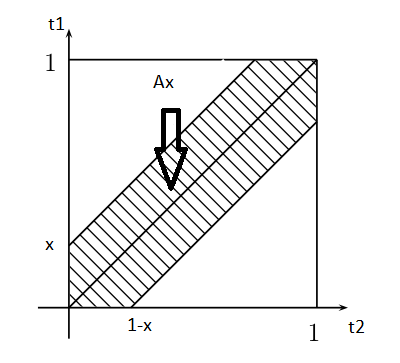
\includegraphics[width=0.5\linewidth]{img/vstr1.png}
		\caption{Задача о встрече}
	\end{figure}

	\begin{gather*}
		\xi((\omega)=(t_1,t_2)) = |t_1 - t_2| \ \ F_{\xi}(x) = \mathbb{P} \{ \xi < x \} = \mathbb{P} \{ \omega \in \Omega : |t_1 - t_2| < x \} = \\
		= \mathbb{P} \left\{\begin{array}{l} \varnothing , x \leq 0 \\ A_x, x \in (0,1)\\ \Omega, x > 1\end{array}\right. =\mathbb{P} \left\{\begin{array}{l} 0 , x \leq 0 \\ 1-(1-x)^2, x \in (0,1)\\ 1, x > 1 \end{array}\right.
	\end{gather*}
\end{zad}

\begin{defs}[Основные дискретные распределения]
	\begin{multicols}{2}
	\begin{itemize}
			\item \zagolovok{Вырожденное}
			\[ \xi \sim \left( \begin{array}{c}
				a \\ \hline
				1 \\
			\end{array} \right) \]
			$\xi \sim \boldsymbol{D}(a)$, $a \in \mathbb{R}$
			\item \zagolovok{Биномиальное}
			$\xi \sim \boldsymbol{Bi}(n,p)$, $n \in \mathbb{N}$, $p \in (0,1)$ -- параметр, $q=1-p$
			\[ \xi \sim \left( \begin{array}{ccccc}
				0 & \multicolumn{1}{|c}{\cdots} & \multicolumn{1}{|c}{k} & \multicolumn{1}{|c}{\cdots} & \multicolumn{1}{|c}{n}\\ \hline
				q^{n} & \multicolumn{1}{|c}{\cdots} & \multicolumn{1}{|c}{\binom{n}{k}p^{k}q^{n-k}} & \multicolumn{1}{|c}{\cdots} & \multicolumn{1}{|c}{p^{n}}\\
			\end{array} \right) \]
			\item \zagolovok{Пуассоновское}
			$\xi \sim \boldsymbol{\Pi}(\lambda)$, $\lambda > 0$ -- параметр,
			\[ \xi \sim \left( \begin{array}{ccccc}
				0 & \multicolumn{1}{|c}{1} & \multicolumn{1}{|c}{\cdots} & \multicolumn{1}{|c}{k} & \multicolumn{1}{|c}{\cdots}\\ \hline
				e^{-\lambda} & \multicolumn{1}{|c}{\lambda e^{-\lambda}} & \multicolumn{1}{|c}{\cdots} & \multicolumn{1}{|c}{\frac{\lambda^{k}}{k!} e^{-\lambda}} & \multicolumn{1}{|c}{\cdots}\\
			\end{array} \right) \]
			\item \zagolovok{Геометрическое}
			$\xi \sim \boldsymbol{G}(p)$, $p \in (0,1)$ -- параметр,
			\[ \xi \sim \left( \begin{array}{ccccc}
				1 & \multicolumn{1}{|c}{2} & \multicolumn{1}{|c}{\cdots} & \multicolumn{1}{|c}{k} & \multicolumn{1}{|c}{\cdots}\\ \hline
				p & \multicolumn{1}{|c}{pq} & \multicolumn{1}{|c}{\cdots} & \multicolumn{1}{|c}{pq^{k-1}} & \multicolumn{1}{|c}{\cdots}\\
			\end{array} \right) \]
	\end{itemize}
	\end{multicols}
\end{defs}

\begin{defs}[Основные абсолютно непрерывные распределения]
	\begin{itemize}
		\item \zagolovok{Равномерное на отрезке}

		\begin{gather*}
			\xi \sim \boldsymbol{R}(a,b), a,b \in \mathbb{R}, a < b: \ \xi \sim f_{\xi}(x) = \levfigurn{0 , x \notin [a,b] \\ \frac{1}{b-a}, x \in [a,b]}; \xi \sim F_{\xi}(x) = \levfigurn{	0 , x \leq a \\ \frac{x-a}{b-a}, a \leq x \leq b \\ 1 , x \geq b}
		\end{gather*}
		\begin{figure}[H]
		      \centering
		      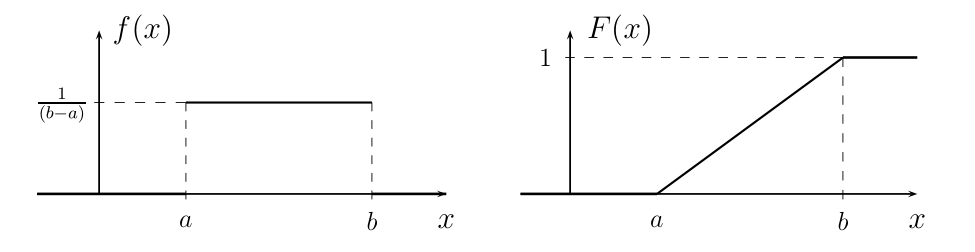
\includegraphics[width=0.8\linewidth]{img/ravnom1.png}
		      \caption{Графики равномерного на отрезке}
		\end{figure}
		\item \zagolovok{Нормальное}

		$$\xi \sim \mathcal{N}(a,\sigma^{2}), a \in \mathbb{R}, \sigma^{2} > 0, \ \sigma = +\sqrt{\sigma^{2}} > 0, \xi \sim f_{\xi}(x) = \frac{1}{\sqrt{2\pi\sigma^{2}}}e^{-\frac{(x-a)^{2}}{2\sigma^{2}}}, \forall x \in \mathbb{R}$$

		\begin{figure}[H]
		      \centering
		      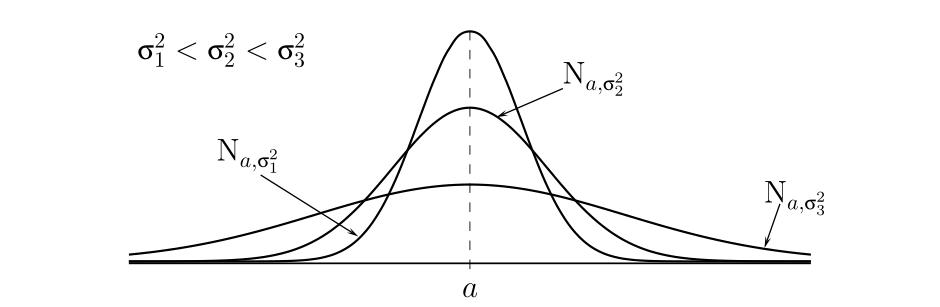
\includegraphics[width=0.8\linewidth]{img/plotnorm.png}
		      \caption{Плотности нормальных распределений}
		\end{figure}

		\begin{figure}[H]
		      \centering
		      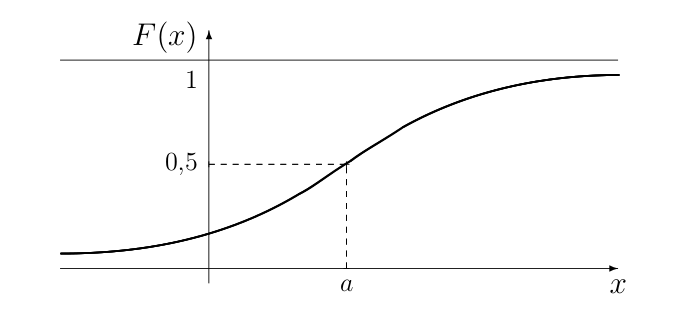
\includegraphics[width=0.8\linewidth]{img/frnorm.png}
		      \caption{Функция распределения нормального распределения $\xi \sim F_{\xi}(x) = \Phi \left( \frac{x-a}{\sigma} \right)$}
		\end{figure}
		Стандартное нормальное распределение:

		$\xi \sim \mathcal{N}(0,1)$

		$\xi \sim f_{\xi}(x) = \frac{1}{\sqrt{2\pi}} e^{-\frac{x^{2}}{2}}$

		$\xi \sim F_{\xi}(x) = \Phi(x) = \int\limits_{-\infty}^{x} \frac{1}{\sqrt{2\pi}} e^{-\frac{t^{2}}{2}} dt$ -- функция Лапласа

		\item \zagolovok{Показательное}

		$\xi \sim \boldsymbol{Exp}(\lambda)$, $\lambda > 0$, $\xi \sim \boldsymbol{Exp}(\lambda) = \boldsymbol{\Gamma}(1, \frac{1}{\lambda})$,
		$\xi \sim f_{\xi}(x) = \levfigurn{	0 , x \leq 0 \\ \lambda e^{-\lambda x}, x > 0}$, $\xi \sim F_{\xi}(x) = \levfigurn{			0 , x \leq 0 \\ 1-e^{-\lambda x}, x > 0}$
		\begin{figure}[H]
		      \centering
		      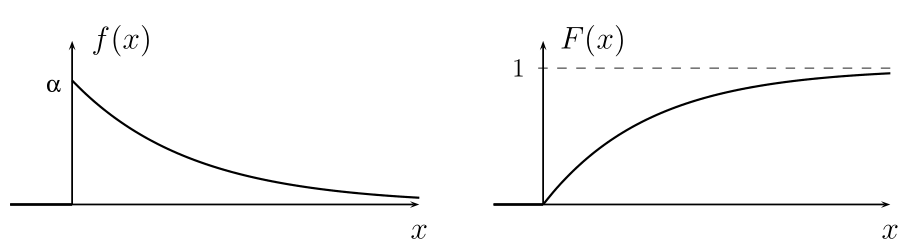
\includegraphics[width=0.8\linewidth]{img/expon.png}
		      \caption{Плотность и функция распределения}
		\end{figure}
		\item \zagolovok{Гамма-распределение}

		$\xi \sim \boldsymbol{\Gamma}(\alpha, \beta)$, $\alpha > 0$, $\beta > 0$
		$\xi \sim f_{\xi}(x) = \levfigurn{	0 , x \leq 0 \\
			\frac{x^{\alpha - 1}}{\Gamma(\alpha) \beta^{\alpha}} e^{-\frac{x}{\beta}}, x > 0}$,

			$\Gamma(\alpha) = \int\limits_{0}^{+\infty} x^{\alpha -1} e^{-x} dx$, $\xi \sim F_{\xi}(x) = \int\limits_{-\infty}^{x} f_{\xi}(t)dt$ -- явно не вычисляется.
			\item \zagolovok{Хи-квадрат-распределение}

			$\xi \sim \boldsymbol{\chi}_{2}^{\alpha} := \boldsymbol{\Gamma}(\frac{\alpha}{2}, 2)$, $\alpha > 0$
			\begin{figure}[H]
			      \centering
			      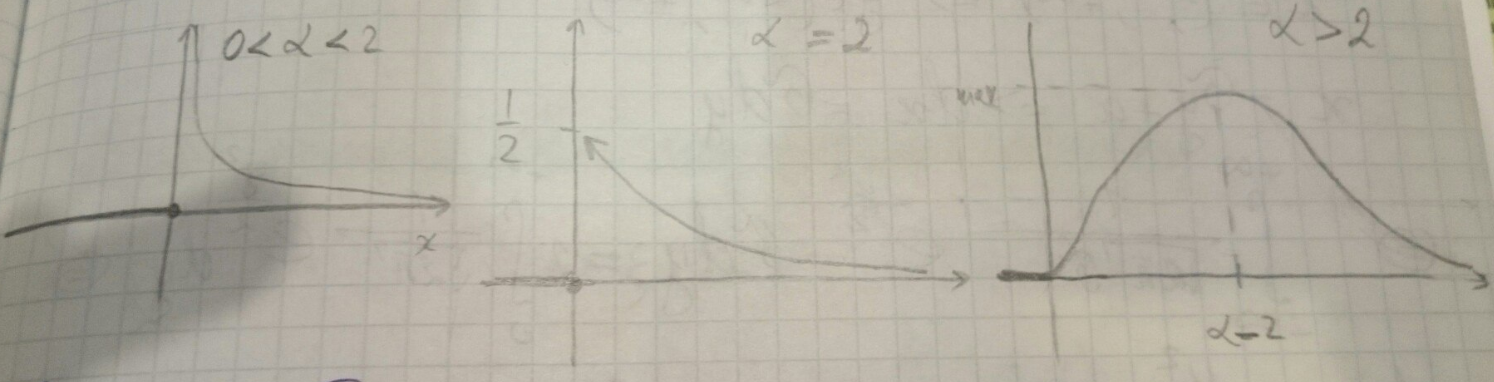
\includegraphics[width=0.8\linewidth]{img/chi.png}
			      \caption{Плотность хи-квадрат-распределения}
			\end{figure}
	\end{itemize}
\end{defs}
\newpage
 %Егор

%Спецчасть
%!TEX root = ../report.tex"
\section{Вопрос 48: Критерий цикличности мультипликативной группы кольца вычетов}

Хорошо известно, что аддитивная группа кольца вычетов $(\mathbb{Z}_{N};+)$ является циклической. Она порождается любым обратимым элементом кольца. Вчастности, $(\mathbb{Z}_{N};+) =\ <1>$. Рассмотрим мультипликативную группу $(\mathbb{Z}^{*}_{N},\cdot)$ этого кольца.
Пусть натуральное число N имеет каноническое разложение $N=\prod_{i=1}^N {p_{i}^{k_{i}}}$. Тогда $$|\mathbb{Z}_{N}^{*}| = \phi(N) = \prod_{i=1}^s {p_{i}^{k_{i}-1}\cdot(p_{i}-1)}$$ и $$ \mathbb{Z}_{N}^{*} \cong \mathbb{Z}_{p_{1}^{k_{1}}}^{*} \otimes \cdots \otimes \mathbb{Z}_{p_{s}^{k_{s}}}^{*}, \eqno(1)$$
где $\otimes$ - операция внешнего прямого произведения групп. Значит, для описания строения группы $\mathbb{Z}_{N}^{*}$ достаточно сделать это лишь для примарных модулей $p_{i}^{k_{i}}$. Для этого нам понадобятся некоторые утверждения о сравнениях по примарным модулям.

\begin{lemma}
	Для любого простого числа $p$, любых $k, t \in \mathbb{N}_{0}$ и $a,b \in \mathbb{Z}$ справедливо следующее: $a \equiv b (mod\ p^{k}) \Rightarrow a^{p^t} \equiv b^{p^t} (mod\ p^{k+t})$
	\begin{dokvo}
		Доказательство производится индукцией по t.
		\begin{enumerate*}
			\item Для $t=0$ утверждение очевидно.
			\item Пусть верно для $t>0$. По предположению индукции $a^{p^t} = b^{p^t}+p^{k+t}c, c \in \mathbb{Z}$. Тогда по формуле бинома Ньютона
			$a^{p^{t+1}}= (b^{p^t}+p^{k+t}c)^p = b^{p^{t+1}}+\binom{p}{1} b^{p^t (p-1)}p^{k+t}c + \binom{p}{2} b^{p^t (p-2)}p^{2(k+t)}c^2 +...$
			Отсюда, учитывая, что $p | \binom{p}{i}$ при $1 \leq i \leq p-1$, получим $a^{p^{t+1}} = b^{p^{t+1}} + p^{k+t+1}(b^{p^{t}(p-1)}c+\frac{p-1}{2}b^{p^{t}(p-2)}p^{k+t-1}c^2+\dots) = b^{p^{t+1}} + p^{k+t+1}c'$
		\end{enumerate*}
		Лемма доказана.
	\end{dokvo}
\end{lemma}

Аналогично, индукцией по t с использованием формулы бинома Ньютона доказываются следующие две леммы.

\begin{lemma}
	Если p - нечетное простое число, $a \in \mathbb{Z}$ и $a = 1 +pc_{0}$, где $(p,c_{0}) = 1$, то $\forall t \in \mathbb{N}_{0}$ имеет место равенство
	$a^{p^{t}} = 1+p^{t+1}c_{t}$, где $(p,c_{t})=1$.
\end{lemma}

\begin{lemma}
	Если $a \in \mathbb{Z}$ и $a = 1 + 2^{2}c_{0}$, где $(2,c_{0}) = 1$, то $\forall t \in \mathbb{N}_{0}$ имеет место равенство
	$a^{2^{t}} = 1+2^{t+2}c_{t}$, где $(2,c_{t})=1$.
\end{lemma}

\begin{proofs}[О строении группы $\mathbb{Z}_{p^{k}}^{*}$ при нечетном простом p]
	$\forall$ нечетных простых p и $\forall$ $k \in \mathbb{N}$ группа $\mathbb{Z}_{p^{k}}^{*}$ является циклической.
	\begin{dokvo}
		Во-первых, заметим, что для $k=1$ группа $\mathbb{Z}_{p^{k}}^{*}$ является мультипликативной группой конечного поля из p элементов, и потому циклическая(решали когда-то на ПЗ такую задачу). При k>1 рассмотрим циклические подгруппы $\mathbb{Z}_{p^{k}}^{*}$:
		\begin{enumerate*}
			\item $A=<a>$, где $a = 1 + pc, (p,c) = 1$
			\item $B=<b^{p^{k-1}}>$, где b выбрано так, что число $b_{1} = r_{p}(b)$ является образующим элементом группы $\mathbb{Z}_{p^{k}}^{*}$. Очевидно, что $(p,b)=1$.
		\end{enumerate*}
		Непосредственно из леммы 1 получаем $a^{p^{k-1}} \equiv 1 (mod\ p^{k})$, $a^{p^{k-2}} \not\equiv 1 (mod\ p^{k})$. Значит, порядок элемента a в группе $\mathbb{Z}_{p^{k}}^{*}$ равен $p^{k-1}$ и, следовательно, $|A| = p^{k-1}$.
		Так как по теореме Эйлера Ферма выполняется сравнение $b^{\phi(p^{k})} \equiv 1 (mod\ p^{k})$, то $(b^{p^{k-1}})^{p-1} \equiv 1 (mod\ p^{k})$.

		Допустим, что $(b^{p^{k-1}})^t \equiv 1(mod\ p^{k})$ при $0 < t < p-1$. Тогда и $(b^{p^{k-1}})^t \equiv 1(mod\ p)$. По малой теореме Ферма $b^{p-1} \equiv 1 (mod\ p)$. Отсюда легко следует сравнение $b^{p} \equiv b (mod\ p)$, а потому и $b^{p^{k-1}} \equiv b (mod\ p)$. Значит, $b^t \equiv b^{t}_{1} \equiv 1 (mod\ p)$, что противоречит выбору b. В итоге мы доказали, что порядок элемента $b^{p^{k-1}}$ в группе $\mathbb{Z}_{p^{k}}^{*}$ равен $p-1$ и, следовательно, $|B| = p-1$.

		Заметим, что $(|A|,|B|) = 1$, и потому $|A \bigcap B|=1$. Значит, AB - прямое произведение подгрупп. При этом $|AB|=|A||B|=p^{k-1}(p-1)=|\mathbb{Z}_{p^{k}}^{*}|$, поэтому $AB = \mathbb{Z}_{p^{k}}^{*}$.
		Воспользуемся теперь тем фактом, что прямое произведение групп G, H является циклической группой $\Leftrightarrow$ G, H - циклические и их порядки взаимно просты.
		Поскольку порядки подгрупп A и B взаимно просты, то группа $AB = \mathbb{Z}_{p^{k}}^{*}$ - циклическая.
	\end{dokvo}
\end{proofs}

\begin{proofs}[О цикличности группы $\mathbb{Z}_{2^{k}}^{*}$]
	При $k \in {1,2}$ группа $\mathbb{Z}_{p^{k}}^{*}$ является циклической. При $k > 2$ группа $\mathbb{Z}_{p^{k}}^{*}$ не является циклической и раскладывается в произведение двух циклических подгрупп порядков 2 и $2^{k-2}$.
	\begin{dokvo}
		При $k \in {1,2}$ утверждение теоремы очевидно.
		Пусть $k > 2$. Обозначим $A = {1, 2^{k}-1}, B = {b \in \mathbb{Z}_{2^{k}}^{*} | b \equiv 1 (mod\ 2^{2})}$. Нетрудно заметить, что A и B - подгруппы в $\mathbb{Z}_{2^{k}}^{*}$. При этом A - циклическая подгруппа порядка 2.

		Представим теперь элементы множества B в двоичной системе счисления $b = \sum_{i=0}^{k-1}b_{i}2^{i}$. Т.к. $b \equiv 1(mod\ 2^2)$, то $b_0 = 1, b_1 = 0$. Значит, все элементы множества B представляются в виде $b = 1 + 2^{2}c, 0 \leq c < 2^{k-2}$. Отсюда, в частности, следует, что $|B| = 2^{k-2}$ и $2^{k}-1 = \sum_{i=0}^{k-1}2^{i} \notin B$.
		Итак, $|A \bigcap B| = 1$, AB - прямое произведение подгрупп, $|AB|=|A||B|=2 \cdot 2^{k-2} = |\mathbb{Z}_{2^{k}}^{*}|$ и $AB = \mathbb{Z}_{2^{k}}^{*}$.

		Докажем, что подгруппа B циклическая. Для этого выберем $b = 1 + 2^{2}c \in B, (2,c)=1$. Непосредственно из леммы 2 получаем соотношения $b^{2^{k-2}} \equiv 1 (mod\ 2^{k}), b^{2^{k-3}} \not\equiv 1(mod\ 2^{k})$.
		Значит, порядок элемента b в группе $\mathbb{Z}_{2^{k}}^{*}$ равен $2^{k-2}$ и, следовательно, $B=<b>$.

		Осталось заметить, что прямое произведение $AB = \mathbb{Z}_{2^{k}}^{*}$ не является циклической группой, поскольку порядки A и B не взаимно просты.
	\end{dokvo}
\end{proofs}

На основании этих двух теорем можно сформулировать следующий критерий.

\begin{proofs}[Критерий цикличности группы $\mathbb{Z}_{N}^{*}$]
	Группа $\mathbb{Z}_{N}^{*}$ является циклической $\Leftrightarrow N \in  \{2,4,p^{k}, 2p^{k}|p$ - нечетное простое число$\}$.
	\begin{dokvo}
		Рассмотрим каноническое представление числа $N = \prod_{i=1}^{s}p_{i}^{k_{i}}$ и разложение (1). Если $s = 1$, то утверждение теоремы следует из предыдущих теорем.
		Пусть теперь $s>1$. Если при этом среди чисел $p_{1},\dots,p_{s}$ существуют два нечетных числа $p_{i}, p_{j}$, то порядки групп $\mathbb{Z}_{p^{k_{i}}_{i}}^{*}$ и $\mathbb{Z}_{p^{k_{j}}_{j}}^{*}$ не взаимно просты (т.к. они чётны). Значит, в этом случае группа $\mathbb{Z}_{N}^{*}$ не циклическая.
		Осталось рассмотреть случай $s=2, p_{1}=2, p_{2}$ - нечетное простое число. Если $k_{1}>2$, то по предыдущей теореме группа $\mathbb{Z}_{2^{k_{1}}}^{*}$ (а, следовательно, и $\mathbb{Z}_{N}^{*}$) не циклическая.
		Если $k_{1}=2$, то группа $\mathbb{Z}_{N}^{*} \cong \mathbb{Z}_{2^{2}}^{*} \otimes \mathbb{Z}_{p_{2}^{k_{2}}}^{*}$ не является циклической, т.к. порядки групп $\mathbb{Z}_{2^{2}}^{*}$ и $\mathbb{Z}_{p_{2}^{k_{2}}}^{*}$ не взаимно просты. Если же $k_{1} = 1$, то порядок группы $\mathbb{Z}_{2}^{*}$ равен единице, и группа $\mathbb{Z}_{N}^{*}$ циклическая.
	\end{dokvo}
\end{proofs}
\newpage
 %Mike

%Модели
%!TEX root = ../report.tex"
\section{Вопрос 56: Модель матрицы доступов Харрисона-Руззо-Ульмана (ХРУ). Теорема об алгоритмической неразрешимости задачи проверки безопасности произвольной системы ХРУ.}

\textbf{Модель ХРУ} реализует дискреционную политику управления доступом:
\begin{enumerate}
	\item Все сущности должны быть идентифициорованны
	\item Задана матрица доступов
	\item Субъект обладает правом доступа к сущности ТИТТК в заданной ячейке есть право доступа
\end{enumerate}

\begin{defs}[Модель ХРУ]
	\begin{enumerate}
		\item О -- множество объектов
		\item S -- множество субъектов
		\item R -- множество видов прав доступа субъектов к объектам (например read, write, own - владеть)
		\item M -- матрица доступов (строки представляют собой субъекты, столбцы - объекты)
	\end{enumerate}
\end{defs}

\begin{figure}[H]
	\centering
	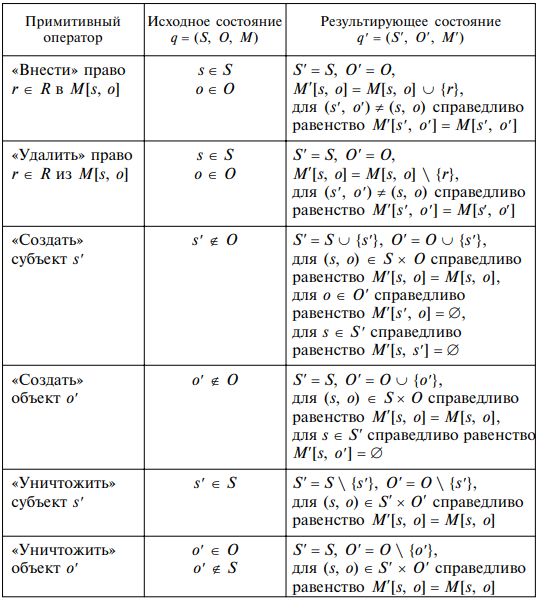
\includegraphics[width=0.5\linewidth]{img/1.png}
	\caption{Табличка}
\end{figure}

\begin{defs}[Утечка права]
	Будем считать, что в состоянии $q$ системы ХРУ возможна утечка права доступа $r \in R$ в результате выполнения команды С$\myvect{1}{n}$ в случае,
	когда при переходе системы $q \vdash_{c(x_1, \ldots, x_k)} q^{\shtrih}$ выполняется примитивный оператор, вносящий право доступа $r$ в ячейку матрицы доступов $M$, до этого $r$
	не содержащую.
\end{defs}

\begin{defs}[Безопасное начальное состояние]
	Начальное состояние $q_0$ системы ХРУ называется безопасным относительно некоторого права доступа $r \in R$ в случае, когда невозможен переход
	системы в такое состояние $q$, в котором возможна утечка права $r$.
\end{defs}

\begin{defs}[монооперационная система ХРУ]
	Система ХРУ называется монооперационной, когда каждая команда системы содержит один примитивный оператор.
\end{defs}

\begin{proofs}
	$\exists$ алгоритм, проверяющий является ли начальное состояние произвольной монооперационной системы ХРУ безопасным относительно некоторого
	права доступа $r \in R$.
\end{proofs}

\begin{proofs}[Об алгоритмической неразрешимости]
	Задача проверки безопасности произвольных систем ХРУ алгоритмически неразрешима.
	\begin{dokvo}
		Из теории машины Тьюринга: не существует алгоритма проверки для произвольной машины Тьюринга (МТ) и произвольного начального слова остановится ли МТ в конечном состоянии или нет.

		Представим все элементы и команды МТ в виде элементов и команд системы ХРУ.

		\textbf{МТ:}

		$ A = \{ \alpha_0, \ldots, \alpha_m \} $ -- внешний авлфавит, $ \alpha_0 = \wedge $ -- пустой символ.

		$ Q = \{ q_0, \ldots, q_k \} $ -- внутренний алфавит, $q_1$ -- начальное состояние, $q_0$ -- конечное.

		$ D = \{ r, l, e \} $ -- множество действий (вправо, влево, на месте).

		$ C: Q \times A \to Q \times A \times D $ -- функция, задающая команды МТ.

		Пусть МТ выполнила некоторое количество шагов. Пусть считывающая головка указывает на ячейку $ i \in \{ 1, \ldots , n \} $. $ (\alpha_{s_{1}}, \ldots, \alpha_{s_{n}}) $ -- заполненные ленты.

		$ R = Q \cup A \cup \{own, left, right \} $

		$ q_{ij} \in M[s_i, s_i] $ -- считывающая головка указывает на ячейку с номером $i$.

		$left \in M[s_1, s_1]$ -- признак крайней левой позиции

		$right \in M[s_n, s_n]$ -- признак крайней правой позиции

		Т.о. построим матрицу доступов:

		\begin{figure}[H]
			\centering
			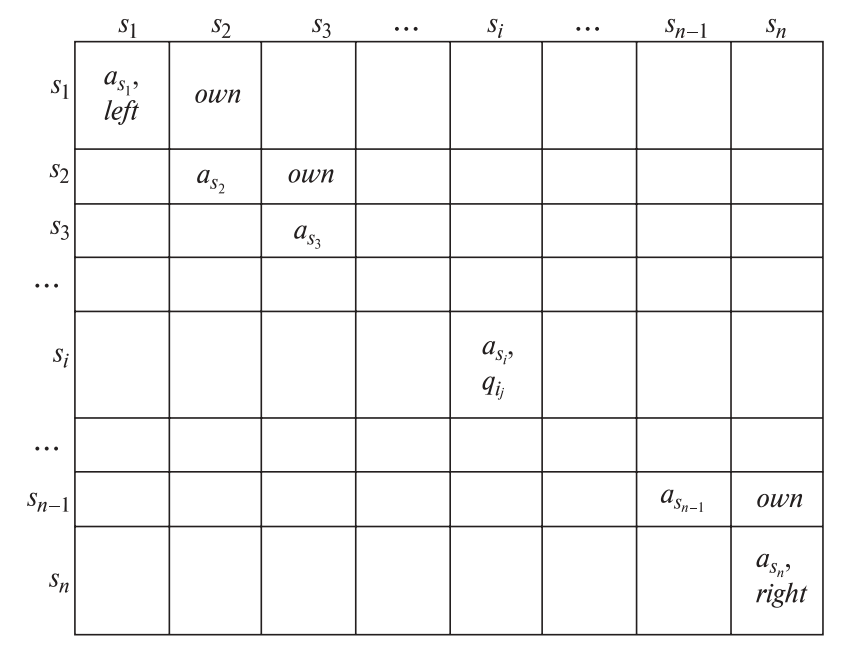
\includegraphics[width=0.5\linewidth]{img/2.png}
			\caption{Матрица доступов}
		\end{figure}

		Построим гомоморфизм машины Тьюринга в систему ХРУ. Зададим каждой команде МТ команду ХРУ:

		Если $d = e$, то

		$command E_{q_{i_{j}}a_{i_{t}}q_{i_{j^{\shtrih}}}a_{i_{t^{\shtrih}}}}(s)$

		$if (q_{i_{j}} \in M[s,s]) and (a_{i_{t}} \in M[s,s]) then $

		\kav{удалить} право $q_{i_{j}}$ из $M[s,s]$

		\kav{удалить} право $a_{i_{t}}$ из $M[s,s]$

		\kav{внести} право $q_{i_{j^{\shtrih}}}$ в $M[s,s]$

		\kav{внести} право $a_{i_{t^{\shtrih}}}$ в $M[s,s]$

		$endif$

		$end$

		Если $d = r$, то 2 случая (для крайней правой позиции и для другой произвольной)

		$command R1_{q_{i_{j}}a_{i_{t}}q_{i_{j^{\shtrih}}}a_{i_{t^{\shtrih}}}}(s, s^{\shtrih})$

		$if (q_{i_{j}} \in M[s,s]) and (a_{i_{t}} \in M[s,s])and (own \in M[s,s^{\shtrih}]) then $

		\kav{удалить} право $q_{i_{j}}$ из $M[s,s]$

		\kav{удалить} право $a_{i_{t}}$ из $M[s,s]$

		\kav{внести} право $a_{i_{t^{\shtrih}}}$ в $M[s,s]$

		\kav{внести} право $q_{i_{j^{\shtrih}}}$ в $M[s^{\shtrih},s^{\shtrih}]$

		$endif$

		$end$

		$command R2_{q_{i_{j}}a_{i_{t}}q_{i_{j^{\shtrih}}}a_{i_{t^{\shtrih}}}}(s, s^{\shtrih})$

		$if (q_{i_{j}} \in M[s,s]) and (a_{i_{t}} \in M[s,s])and (right \in M[s,s]) then $

		\kav{удалить} право $q_{i_{j}}$ из $M[s,s]$

		\kav{удалить} право $a_{i_{t}}$ из $M[s,s]$

		\kav{удалить} право $right$ из $M[s,s]$

		\kav{внести} право $a_{i_{t^{\shtrih}}}$ в $M[s,s]$

		\kav{создать} субъект $s^{\shtrih}$

		\kav{внести} право $own$ в $M[s,s^{\shtrih}]$

		\kav{внести} право $a_0$ в $M[s^{\shtrih},s^{\shtrih}]$

		\kav{внести} право $q_{i_{j^{\shtrih}}}$ в $M[s^{\shtrih},s^{\shtrih}]$

		\kav{внести} право $right$ в $M[s^{\shtrih},s^{\shtrih}]$

		$endif$

		$end$

		Аналогично для $d = l$. Из алгоритмической неразрешимости проверки, остановится ли МТ в своем конечном состоянии или нет следует
		алгоритмическая неразрешимость задачи проверки безопасности системы ХРУ.
	\end{dokvo}
\end{proofs}
 %Владка
%!TEX root = ../report.tex"
\section{Вопрос 57: Модель распространения проав доступа Take-Grant. Теорема о передаче прав в графе доступов, состоящем только из субъектов, и в произвольном графе доступов. Сведение систем Take-Grant к системам ХРУ и ТМД.}

\textbf{Модель $Take-Grant$} ориентирована на анализ путей распространения прав доступа в системах дискреционного управления доступом.

\begin{defs}[Модель $Take-Grant$]
	\begin{enumerate*}
		\item $ O $ -- множество объектов.
		\item $S \subseteq O$ -- множество субъектов.
		\item $ R = \{ r_1, \ldots, r_m \} \cup \{ t, g \} $ -- множество видов прав доступа, где t -- право брать права доступа, g -- давать.
		\item $ G = (S, O, E) $ -- конечный, ориентированный без петель граф доступов, $E \subseteq O \times O \times R $ -- ребра графа.
	\end{enumerate*}
\end{defs}

\textbf{Цель модели} -- определение и обоснование условий проверки возможности утечки права доступа по исходному графу.

\begin{defs}[Предикат $can-share$]
	$ \sqsupset x,y \in O_0, G_0 = (S_0, O_0, E_0), \alpha   \subseteq R$. Определим предикат
	$can-share(\alpha, x, y, G_0)$, который истинен ТИТТК $ \exists G_1 = (S_1, O_1, E_1), \ldots,
	G_N = (S_N, O_N, E_N)$ и правила $op_1, \ldots, op_N, N \geqslant 0$, т.что
	$G_0 \vdash_{op_1} \ldots \vdash_{op_N} G_N $ и $(x, y, \alpha) \subset E_N$.
\end{defs}

\begin{defs}[$tg$-связность]
	Пусть $G = (S, S, E)$ -- граф доступов, вершины которого являются субъектами. Вершины являются $tg$-связными, или
	соединены $tg$-путем, если между ними существует путь, каждое ребро которого помечено t или g.
\end{defs}

\begin{proofs}[О передаче прав в графе только из субъектов]
	$\sqsupset  G_0 = (S_0, S_0, E_0), x,y \in S_0, x \neq y$. Тогда предикат $can-share(\alpha, x, y, G_0)$
	истинен ТИТТК выполняются условия:
	\begin{enumerate*}
		\item $ \sqsupset s_1, \ldots, s_m \in S_0 : (s_i, y, \gamma_i) \subset E_0 $, где
		$ i = 1, \ldots, m $ и $ \alpha = \gamma_1 \cup \ldots \cup \gamma_m $.
		\item Субъекты $ x $ и $ s_i $ являются $tg$-связными в графе $G_0, i = 1, \ldots, m $.
	\end{enumerate*}
\end{proofs}

\begin{defs}[Остров]
	Островом в произвольном графе доступов $G_0$ называется его максимальный tg-связный подграф, состоящий только из вершин субъектов.
\end{defs}

\begin{defs}[Мост]
	Мостом в графе доступов $G_0$ называется tg-путь, концами которого являются вершины субъекты, проходящий через вершины объекты.
\end{defs}

\begin{defs}[Начальный пролет]
	Начальным пролетом моста в графе доступов называется tg-путь, началом которого является вершина субъект, концом -- объект, проходящий через ввершины объекты, словарная запись которого имеет вид
	 $ \overrightarrow{t}^* \overrightarrow{g} $.
\end{defs}

\begin{defs}[Конечный пролет]
	Конечным пролетом моста в графе доступов называется tg-путь, началом которого является вершина субъект, концом -- объект, проходящий через ввершины объекты, словарная запись которого имеет вид
	$\overrightarrow{t}^*$.
\end{defs}

\begin{proofs}[О передаче прав в произвольном графе]
	$\sqsupset  G_0 = (S_0, O_0, E_0), x,y \in O_0, x \neq y$. Тогда предикат $can-share(\alpha, x, y, G_0)$
	истинен ТИТТК или $(x, y, \alpha ) \subset E_0$, или выполняются условия:
	\begin{enumerate*}
		\item $ \sqsupset s_1, \ldots, s_m \in O_0 : (s_i, y, \gamma_i) \subset E_0 $, где
		$ i = 1, \ldots, m $ и $ \alpha = \gamma_1 \cup \ldots \cup \gamma_m $.
		\item $ \exists x_1^{\shtrih}, \ldots, x_m^{\shtrih}, s_1^{\shtrih}, \ldots, s_m^{\shtrih} \in S_0$ :
			\begin{itemize*}
				\item $x = x_i^{\shtrih}$ или $x_i^{\shtrih}$ соединен с $x$ начальным пролетом моста в графе $G_0$
				\item $s_i = s_i^{\shtrih}$ или $s_i^{\shtrih}$ соединен с $s_i$ конечным пролетом моста в графе $G_0$
			\end{itemize*}
		\item В графе $G_0$ для каждой пары $(x_i^{\shtrih}, s_i^{\shtrih}) \exists $ острова $I_{i,1}, \ldots, I_{i, u_{i}}$, где $u_i \geqslant 1$, т.что
		$x_i^{\shtrih} \in I_{i,1}, s_i^{\shtrih} \in I_{i, u_{i}}$, и существуют мосты между островами $I_{i,j}$ и $I_{i, j+1}, j = 1, \ldots, u_i - 1$.
	\end{enumerate*}
\end{proofs}

\textbf{Take-Grant в ХРУ}

Состояние системы $Take-Grant$ описыается:
\begin{enumerate*}
	\item $G=(S_{tg}, O_{tg}, E)$
	\item $R_{tg}$
\end{enumerate*}

\textbf{ХРУ:}
\begin{enumerate*}
	\item $R = R_{tg} \cup \{own\}$
	\item $S = O = O_{tg}$
	\item $M_{|S| \times |S|}$ -- матрица доступов, если $(x,y,r) \in E$, то $r \in M[x,y]$, для $s \in S_{tg}$ выполняется условие $own \in M[s,s]$
\end{enumerate*}

\begin{multicols}{2}
	\begin{itemize*}
		\item $\mathbf{command} \  Take_{\alpha}(x,y,z)$

		$if (own \in M[x,x]) and (t \in M[x,y])and (r_1 \in M[y,z])and  \ldots and (r_k \in M[y,z]) then $

		\kav{внести} право $r_1$ в $M[x,z]$

		$\ldots$

		\kav{внести} право $r_k$ в $M[x,z]$

		$endif$

		$end$

		\item 		$\mathbf{command} \  Grant_{\alpha}(x,y,z)$

				$if (own \in M[x,x]) and (g \in M[x,y])and (r_1 \in M[x,z])and  \ldots and (r_k \in M[x,z]) then $

				\kav{внести} право $r_1$ в $M[y,z]$

				$\ldots$

				\kav{внести} право $r_k$ в $M[y,z]$

				$endif$

				$end$
		\end{itemize*}
		\begin{itemize*}
		\item 		$\mathbf{command} \ CreateObjectAlpha(x,y)$

				$if (own \in M[x,x]) then $

				\kav{создать} субъект $y$

				\kav{внести} право $r_1$ в $M[x,y]$

				$\ldots$

				\kav{внести} право $r_k$ в $M[x,y]$

				$endif$

				$end$

		\item 		$\mathbf{command} \ CreateSubjectAlpha(x,y)$

				$if (own \in M[x,x]) then $

				\kav{создать} субъект $y$

				\kav{внести} право $own$ в $M[y,y]$

				\kav{внести} право $r_1$ в $M[x,y]$

				$\ldots$

				\kav{внести} право $r_k$ в $M[x,y]$

				$endif$

				$end$
			\end{itemize*}
			\begin{itemize*}

			\item 		$\mathbf{command} \ RemoveAlpha(x,y)$
					$if (own \in M[x,x]) then $

					\kav{удалить} право $r_1$ в $M[x,y]$
					$\ldots$
					\kav{удалить} право $r_k$ в $M[x,y]$

					$endif$

					$end$

	\end{itemize*}

\end{multicols}

\textbf{Take-Grant в ТМД}

	\textbf{Take-Grant:}
	\begin{multicols}{2}
		\begin{enumerate*}
			\item $G=(S_{tg}, O_{tg}, E)$
			\item $R_{tg}$
		\end{enumerate*}
	\end{multicols}

	\textbf{ТМД:}

	\begin{multicols}{2}
		\begin{enumerate*}
			\item $R = R_{tg}$
			\item $S = O = O_{tg}$
			\item $M_{|S| \times |S|}$ -- матрица доступов, где для $x,y \in O_{tg}$,если $(x, y, r) \in E$ то $r \in M[x,y]$
			\item $T = \{subject, object\}$ -- множество типов
			\item $t: O \to T : t(s) = subject, t(o) = object, o \in O_{tg} \backslash S_{tg}$
			\item $q = (S, O, t, M)$ -- состояние ТМД
		\end{enumerate*}
	\end{multicols}



	Построим отображение правил преобразования графов доступов в множество команд системы ТМД.
\begin{multicols}{2}
	\begin{itemize*}
		\item 	$\mathbf{command} \ \mathit{Take}_{r_1, \ldots, r_k}os(x: subject,y:object,z:subject)$

			$if (t \in M[x,y]) \ and (r_1 \in M[y,z])and  \ldots \ and \ (r_k \in M[y,z]) then $

			\kav{внести} право $r_1$ в $M[x,z]$

			$\ldots$

			\kav{внести} право $r_k$ в $M[x,z]$

			$endif$

			$end$

			\item $\mathbf{command} \  \mathit{Grant}_{r_1, \ldots, r_k}so(x: subject,y:subject,z:object)$

			$if (g \in M[x,y]) \ and  \ (r_1 \in M[x,z]) and  \ldots and (r_k \in M[x,z]) \ then $

			\kav{внести} право $r_1$ в $M[y,z]$

			$\ldots$

			\kav{внести} право $r_k$ в $M[y,z]$

			$endif$

			$end$
	\end{itemize*}

	\begin{itemize*}
		\item 		$\mathbf{command} \  \mathit{CreateObjectAlpha}_{r_1, \ldots, r_k}(x: subject,y:object)$


				\kav{создать} субъект $y$ с типом $object$

				\kav{внести} право $r_1$ в $M[x,y]$

				$\ldots$

				\kav{внести} право $r_k$ в $M[x,y]$

				$endif$

				$end$
				\item		$\mathbf{command} \ \mathit{CreateSubjectAlpha}_{r_1, \ldots, r_k}(x: subject,y:subject)$

						$if (own \in M[x,x]) then $

						\kav{создать} субъект $y$ с типом $subject$

						\kav{внести} право $r_1$ в $M[x,y]$

						$\ldots$

						\kav{внести} право $r_k$ в $M[x,y]$

						$endif$

						$end$
	\end{itemize*}
\end{multicols}


		$\mathbf{command} \ \mathit{RemoveAlpha}_{r_1, \ldots, r_k}(x: subject,y:object)$

		$if (own \in M[x,x]) \ then $

		\kav{удалить} право $r_1$ в $M[x,y]$

		\kav{удалить} право $r_k$ в $M[x,y]$

		$endif$

		$end$
\newpage
 %Владка
\end{document}

%%
%%
%%
